\documentclass{upy-report}

% Markup for tracking changes and revisions
% \added[id=<id>, comment=<comment>]{<new text>}
% \deleted[id=<id>, comment=<comment>]{<old text>}
% \replaced[id=<id>, comment=<comment>]{<new text>}{<old text>}
% \highlight[id=<id>, comment=<comment>]{<text>}
% \comment[id=<id>]{<comment>}
\usepackage[]{changes}
\definechangesauthor[name={Gonzalo Peraza}, color=green]{GP}
\setuptodonotes{inline}

% load any additional packages
\usepackage{listings}
\usepackage{booktabs} % to enable the use of \toprule, \midrule, \bottomrule in tables
\usepackage{siunitx} % to use the scientific notation
\sisetup{output-exponent-marker=\ensuremath{\mathrm{e}}} % configuration of the siunitx package to use the "e" notation

%end the preamble and start the document
\begin{document}

% \maketitle                  % create a title page from the preamble info
\begin{titlepage}
	\pdfbookmark[0]{Titlepage}{Titlepage}

	\centering

	% {\Large } \\[4mm]
	
\includegraphics[width=6cm]{Figures/logo} \\[2mm]
	\textsf{Internship Report} \\
	\textsf{Submitted for the degree of} \\
	\textsf{Data Engineer} \\

	\vfill
	% {\large \thesisSubject} \\[5mm]

	{\LARGE \textbf{Universidad Politécnica de Yucatán} \\
	\LARGE  Characterization of the urban road network of Merida, Yucatan, Mexico.  \\[10mm]}

	{\Large Alejandro De Jesus Puerto Castro} \\

	\vfill
	\begin{minipage}[t]{.27\textwidth}
		\raggedleft
		\textit{1. External Supervisor}
	\end{minipage}
	\hspace*{15pt}
	\begin{minipage}[t]{.65\textwidth}
		{\Large Gonzalo G. Peraza Mues} \\
	  	{\small Data Engineering} \\[-1mm]
		{\small Universidad Politécnica de Yucatán}
	\end{minipage} \\[5mm]
	\begin{minipage}[t]{.27\textwidth}
		\raggedleft
		\textit{2. Internal Supervisor}
	\end{minipage}
	\hspace*{15pt}
	\begin{minipage}[t]{.65\textwidth}
		{\Large Didier O. Gamboa Angulo} \\
	  	{\small Data Engineering} \\[-1mm]
		{\small Universidad Politécnica de Yucatán}
	\end{minipage} \\[10mm]
	% \begin{minipage}[t]{.27\textwidth}
	% 	\raggedleft
	% 	\textit{Supervisors}
	% \end{minipage}
	% \hspace*{15pt}
	% \begin{minipage}[t]{.65\textwidth}
	% 	\thesisFirstSupervisor\ and \thesisSecondSupervisor
	% \end{minipage} \\[10mm]

	\today \\

\end{titlepage}

\frontmatter
\pagestyle{empty}

\tableofcontents
\listoffigures
\listoftables

\chapter{Acknowledgments}
\label{cha:acknowledgments}


  % include an acknowledgements.tex file
\chapter{Abstract}


\label{cha:abstract}
          % include the abstract

\mainmatter
\pagestyle{headings}

%now include the files of latex for each of the chapters etc
\chapter{Introduction}
\label{cha:introduction}

Urban planning is crucial for a city to successfully grow. Cities face many challenges day-by-day, and such challenges change, evolve, or are resolved in different eras in the history of the city. The planning includes various processes such as determining land use, arrangement and designing of buildings, transport systems, public spaces, and street (or road) networks. The quality of the environment that is built, has direct impact on the life quality of the people in the community.

Street network analysis has become a common subject in the urban planning literature in the last years. It is also an important bridge between graph theory and urban morphology and planning. For such reason, street network analysis serves as a complementary guide to urban planning.

The capital of Yucatán: Mérida, -- the first safest city in Mexico, and ranked as second in North America by a business magazine \cite{ceoworldmag_2019}--, is a city that has been growing rapidly with insufficient planning, vast investment and disproportionate increase in vehicular traffic in the last years. Such challenges are result of the lack of planning in the city by the governmental authorities.

In this work, we use street network analysis to have some understanding on the morphology of Mérida. The results of the analysis can be used to complement urban planning and improve life quality of the people.

\section{Background}

Mérida is the capital and the most populated municipality in Yucatán. It is located in the northwestern region of the Yucatan Peninsula, with an estimated population of 995,129 inhabitants in an area of 874.4 km$^2$.

Recently, the Municipal Institute of Planning of Mérida (IMPLAN) has made two plans regarding urban development and mobility \cite{PMDU_2017, PIMUS_2019}. Such studies mention that the urban structure and morphology have direct implications on connectivity and accessibility of roads. However, their statements are based on urban studies, and not based on network theory.

\section{Problem Statement} 

Currently, there are no local studies regarding network theory and urban roads in Mérida, along with socio-demographic data. This lack of research, makes us missing an important and insightful point of view of the urban street network in Mérida. Therefore, it exists a necessity for analyzing the urban street network based on network theory in Mérida, Yucatán.

\section{Justification}

We believe that analyzing street network at municipal and AGEB scale with socio-demographic data, will give us a clearer view of the urban form and the topological and metric complexity of the street network. 


\section{Scope and limitations}

This work covers the area of Mérida, Yucatán, México municipality and its urban AGEBs. Also, we only select relevant street network measures based on a review of spatial networks analysis and the study \cite{boeing_multi-scale_2018} made by Boeing. However, the precision of the street network is limited by the contributions in Open Street Map. Additionally, we do not have enough information regarding the analysis of Mérida's street network, as we believe is the first study of its kind in Mérida.

This project, due to its own complexity, was limited by time, human, and computational resources.

\begin{itemize}
	\item \textbf{Time}: This project was set to have a duration of sixteen weeks. Starting on January 4th and ending on April 30th, 2021. We had approximately 640 working hours to finish the project.
	\item \textbf{Human}: The project was done in its entirety by a single Data Engineering student, with the support and supervision of two professors of the Universidad Politécnica de Yucatán's Data Engineering department.
	\item \textbf{Computational}: The project was run on a laptop with a 2-core CPU and 8 GB of RAM. The nature of the calculations require a computer with better specifications.
\end{itemize}

\section{Objectives}
\subsection {General}
 
Obtention and characterization of the urban street network of Mérida, Yucatán, México.
 
\subsection {Specific}

\begin{enumerate}
\item Obtention and characterization of the urban street network of Mérida, Yucatán, México at municipal scale.
\begin{enumerate}
    \item Make an analysis of the current state of feasible tools and services that allows the obtention and characterization of street networks.
    \item Download and model the street network of Mérida, Yucatán, México.
    \item Review relevant measures for spatial networks analysis.
    \item Calculate and describe measures on the street network.
\end{enumerate}


\item Obtention and characterization of the urban street network of Mérida, Yucatán, México at AGEB scale.
\begin{enumerate}
	\item Obtain socio-demographic data of Mérida.
	\item Obtain geometries of the urban AGEBs of Mérida.
	\item Download and model street network for every urban AGEB in Mérida.
	\item Review relevant measures for spatial networks analysis.
	\item Calculate and describe measures on the AGEBs street networks.
	\item Merge street network calculations and socio-demographic data.
\end{enumerate}


\item Identification of AGEBs with similar characteristics. 
\begin{enumerate}
	\item Construct an adjacency matrix based on spatial weights to interconnect AGEBs.
	\item Identify the pertinent clustering algorithm based on the data we are using.
	\item Find the appropiate number of clusters that best similarity between AGEBs.
\end{enumerate}
\end{enumerate}



\chapter{Theoretical framework}
\label{cha:chapter 2}

On this section we present concepts to support and further explain the technologies and process found on the Methodology and Development section. We present concepts regarding spatial networks and its analysis measures based on network theory; spatial data; as well as some tools and services that we use as a base for this work.

\section{Spatial Networks}
A network (or \textit{graph} in mathematics) is composed of nodes $N$ connected by links, or edges, $E$. Nodes represent entities in a network, such as cities, people, airports, and street intersections. Edges represent relationship between nodes, such as friendships among people, flights between airports, street roads, and so on. 

Graphs can be arranged nonspatially or spatially. Spatial graphs have nodes that are georeferenced, i.e. they are defined by their location in geographic space using a pair of coordinates; usually embedded in a two- or three-dimensional space \cite{barthelemy_spatial_2011}. Both nonspatial and spatial graphs can contain undirected, directed, unweighted, or weighted components \cite{anderson_2020}.

An undirected graph has edges that can be used to represent flows of traffic on two-way streets, while edges in a directed graph represent one-way streets. A self-loop in a graph is an edge that connects a single node to itself. Two nodes can also be connected by parallel edges, in such case, graphs are called multigraphs, or multidigraphs if they are directed. The weight attribute in a weighted graph is used to quantify some value between connected nodes \cite{boeing_osmnx_2017}.

Network science was founded on the based on the findings by Euler \cite{euler_1741}, and gave way to the notion that graphs have different structural properties that can be discovered and cataloged using graph theory \cite{barabasi_2016}. With this, early spatial network analysis focused on using graph theory and its measures to describe and catalog the properties of real systems represented as spatial networks \cite{anderson_2020}. 

Real spatial networks are complicated physical entities, with numerous, often complex, elements with a nontrivial configuration and structure that are neither purely fully regular nor fully random. A street network is an example of a complex spatial network with both nodes and edges embedded in space.

A spatial network is \textit{planar} if it can be represented in two dimensions with its edges intersecting only nodes. A street network may be planar at certain small scales, but most street networks are non-planar due to overpasses, bridges, tunnels, etc. For tractability, these networks are studied as approximately planar. However, it can cause analytical problems due to the over-simplification.

Street networks can be based on two graph representations: primal graph or dual graph. In a primal graph representation, intersections are turned into nodes and street segments into edges. On the other hand, dual graphs invert the representation: streets as nodes and intersections as edges \cite{porta_streets_2006}. Primal graphs retain all the geographic, spatial information that are lost in a dual graph. For that reason, primal representation is the better approach for analyzing spatial networks as it faithfully represents all the spatial characteristics of a street \cite{ratti_spacesyntax_2004}.

\section{Spatial Networks Analysis Measures}

The structure and behavior of networks can be described using a variety of graph theory measures. These measures can be found in different level of detail in \cite{barabasi_2016, barthelemy_spatial_2011, lewis_2011, newman_2004, newman_2010, menczer_fortunato_davis_2020}.

Each network is characterized by the \textbf{total number of nodes} $N$ and the \textbf{total number of edges} $E$. We call $N$ the \textbf{size of the network}. 

The \textbf{\textit{degree}} $k$ of a node is its number of edges, or neighbors, and it is a local measure. We use $k_i$ to denote the degree of node $i$. A node with no neighbors has degree zero ($k = 0$) and is called a \textbf{\textit{singleton}}.

The \textbf{average degree} $<k>$ is a global measure for the average degree $k$ across all nodes $N$ in a graph. This measure is simplified by dividing twice the number of edges $E$ by the number of nodes $N$, as follows:

\begin{equation} \label{eq:1}
<k> = \frac{2E}{N}
\end{equation}

The average streets per node measures the mean number of streets (edges in an undirected graph) that come out from each intersection or dead-end.

The \textbf{degree distribution} $P(k)$ represents the fraction of nodes in a graph with degree $k$, calculated by dividing the number of nodes with degree $k$ by the total number of nodes $N$ in the graph $G$. The degree distribution $P(k)$ is often plotted on a histogram and is useful for providing an overall snapshot of graph $G$.

The \textbf{clustering coefficient} $C$ measures the ability of an individual node $i$ to associate with other nodes (cliquishness). It is commonly described as the probability that "friends" of $i$ (i.e., nodes connected to node $i$) are also friends of each other: the chance that a friend of my friend is also my friend \cite{watts_strogatz_1998}. For node $i$ of degree $k_i$, the clustering coefficient $C(i)$ is defined as:

\begin{equation} \label{eq:2}
	C(i) = \frac{E_i}{k_i(k_i - 1)/2}
\end{equation}

where $E_i$ is the number of edges existing between the neighbors of $i$. When the local measure $C = 1$, the node $v_i$ and its neighboring nodes are all perfectly connected. In contrast, when $C = 0$, neighbors of node $i$ are not connected at all.

The \textbf{average clustering coefficient} $<C>$ is a global measure that determines the cliquishness of all nodes in a graph and is calculated as the average $C$ over all individual nodes. When $<C> = 1$, the graph is perfectly connected. In contrast, when $<C> = 0$, the graph is not connected at all.

A \textbf{path} $P$ is and ordered sequence, or collection, of edges that connects some ordered sequence of nodes. The collection of nodes $N$ and edges $E$ in a path can be defined as:

\begin{equation} \label{eq:3}
N_p = \{0,1,2,...n\}
\end{equation}

\begin{equation} \label{eq:4}
E_p = \{0,1,2,...m\}
\end{equation}

There may be many paths of varying lengths $l$ between two nodes $i$ and $j$. The \textbf{shortest path length} $l_s$ is calculated by counting the total number of intermediate nodes or edges along the shortest path between two nodes $i$ and $j$ and is defined as:

\begin{equation} \label{eq:5}
	l_s(i,j) = \min_\text{paths}({i \to j})
\end{equation}

The \textbf{average shortest path length} $<l>$ is defined as the average shortest path length between all possible pairs of nodes in the network. {\textbf{Eccentricity} of a node is the largest distance (the maximum of the shortest-path weighted distances) between a node and other nodes i.e., how far the node is from the node that is furthest from it \cite{urban-keitt_2001}. The \textbf{diameter} of a network is the maximum eccentricity of any node in the network and the \textbf{radius} is the minimum eccentricity \cite{hage-harary_1995}. The \textbf{center} if a network is the node or set of nodes with an eccentricity equals the radius, and the \textbf{periphery} of a network is the node or set of nodes with eccentricity equals the diameter. These distances serve as indicators for network size and shape if we use length as weight.

\textbf{Average street length} is the mean edge length measured in meters, an example of spatial units, and indicates how fine-grained (small block size) or coarse-grained (large block size) the networks is.

Density measures provided how fine-grained the network is. \textbf{Node density} is the number of nodes divided by the area covered by the network. \textbf{Intersection density} is the node density of the set of nodes with more than one street emanating from them, excluding dead-ends. The \textbf{edge density} is the sum of all edge lengths divided by the area. The physical \textbf{street density} is the sum of all edges (in the undirected graph) divided by the area.

The {\textbf{average circuity} is the sum of edge lengths divided by the sum of straight-line distances between edge endpoints \cite{giacomin-levinson_2015}.

\textbf{Connectivity} measures the minimum number of nodes or edges that must be removed from a connected graph to disconnect the network \cite{urban-keitt_2001}. In the case of street networks, we use \textbf{average node connectivity} as a resilience indicator, which is the mean of local node connectivity between each pair of nodes. This measure is more useful to represent the expected number of nodes that must removed to disconnect a randomly selected pair of non-adjacent nodes \cite{beineke-oellermann-pippert_2002, dankelmann-oellermann_2003} Networks with low connectivity may have multiple points of failure, this yield to a vulnerable system. 

Centrality measures indicate the most important nodes in a network \cite{huang_2016, zhong_2017}. \textbf{Betweenness centrality} $g_i$ measures the total number of shortest paths between any two nodes in the graph that pass through node $i$ \cite{freeman_1997, ermagun-levinson_2017} and is defined as:

\begin{equation} \label{eq:6}
g_i = \sum_{u \neq v} \frac{\sigma_{uv} (i)}{\sigma_{uv}}
\end{equation}

where $\sigma_{uv}$ is the number of shortest paths going from node $u$ to note $v$ and $\sigma_{uv}(i)$ is the number of shortest paths going from node $u$ to node $v$ through node $i$. The importance of an edge $j$ is also measured by betweenness centrality $g_j$ that instead calculates the total number of shortest paths between any two nodes in a graph that include edge $j$ \cite{newman_2003} and is defined as:

\begin{equation} \label{eq:7}
g_j = \sum_{u \neq v} \frac{\sigma_{uv} (j)}{\sigma_{uv}}
\end{equation}

where $\sigma_{uv}$ is the number of shortest paths going from node $u$ to node $v$ and $\sigma_{uv}(j)$ is the number of shortest path going from node $u$ to node $v$ through edge $j$. In many graphs, betweenness centrality $g_i$ and node degree $k_i$ correlate, where the most central node can also have the most connections. The \textbf{average betweenness centrality} is the mean of betweenness centralities of all the nodes in the network \cite{barthelemy_spatial_2011}. The maximum betweenness centrality in a network specifies the proportion of shortest paths that pass through the most important node. If the maximum betweenness centrality is high, the network is more susceptible to failure or inefficiency.

\textbf{Closeness centraltity} is another way to measure the centrality of a node by determining how close a node is to the other nodes. This can be done by averaging the sum of the distances from the node to all others. This measure gives low values for more central nodes and high values for less central ones \cite{newman_2010}. It is defined as the inverse of the sum of distances of a node from all others:

\begin{equation} \label{eq:8}
g_i = \frac{1}{\sum_{j \neq i} l_{ij}}
\end{equation}

where $l_{ij}$ is the distance from $i$ to $j$ and the sum runs over all the nodes of the network, except $i$ itself. An alternative formulation to discount the graph size and make the measure comparable across different networks is obtained by multiplying equation \ref{eq:8} by the constant $N - 1$, which is just the number of terms in the sum at the denominator:

\begin{equation} \label{eq:9}
\tilde{g}_i = (N - 1)g_i
\end{equation}

Finally, \textbf{PageRank} is an algorithm to compute a centrality measure that aims to capture the prestige or importance of each node and it is typically used in directed networks. It ranks nodes based on the structure of incoming links and the rank of the source node. This measure can also be applied to street networks \cite{jiang_2006, agryzkov_2012, gleich_2014, chin-wen_2015}. It is worth to mention that multiple studies use centrality measures in combination to assess street networks (e.g., \cite{porta_2004, porta_2006, porta_2010, crucitti_urban_2006, crucitti_spatial_2006, sevtsuk_2012}).

A graph community is defined as a set of nodes that have more connections among themselves than other nodes in the graph \cite{fortunato_2010}. This feature is important in spatial networks since dense connections tend to take place between nodes that are closer in proximity. Moreover, this implies that the majority of flows between nodes occur as a function of nodes belonging to the same geographical region \cite{barthelemy_2018}.

The above measures do not account for the distance between linked node pairs, an important measure that can be used to quantify real spatial networks embedded in geographic space. Distance can be measured in a variety of ways, the most common being Euclidean distance $d_E(i, j)$ or as the direct distance between two points. In contrast, the route distance $d_R(i, j)$ is computed by summing the geographical length of edges, which make up the shortest path between node $v_i$ and $v_j$ \cite{anderson_2020}.

\section{Spatial Data}

Spatial data is embedded in space, whether in a 3D or 2D representation. Data used in this work is encoded as a spatial graph with points, lines, and polygons embedded in space to represent them in the geographical space such as in a map. For such reason, we first need to understand the properties of the space and its representations.

\subsection{Coordinate Reference Systems}

Sometimes the Earth is assumed to have an spherical shape who is described by two coordinates, latitude (north) and longitude (east). However the Earth is not a sphere; its shape is more like an ellipsoid. There are many possible approximations to this shape (called datums), which define their own latitude-longitude coordinate system. A coordinate system (CS) is a sequence of coordinate axes with specified units of measure, and its types are: ellipsoidal, Cartesian, affine, gravity-related, linear, spherical, polar, and cylindrical. A coordinate reference system (CRS) associates a CS with an object by mean of a datum (see Figure \ref{fig:crs-datum}) \cite{nikolli_CRS_2011}. Some are more accurate than others for particular regions of the Earth's surface.  If our data is notated in different datums then we will need to convert them into one standard format. The most common global datum is called WGS84 (World Geodetic System, 1984) \cite{fox_spatial_2018}.

\begin{figure}[h!]
	\centering
	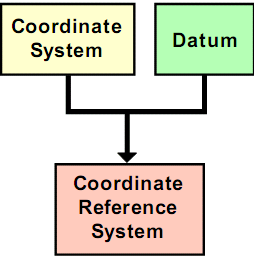
\includegraphics[width=0.3\textwidth]{Figures/coordinate system-datum_nikolli2011.png}
	\caption{A coordinate reference system combines a coordinate system with a datum, which gives the relationship of the coordinate system to the surface and shape of the Earth. Retrieved from \cite{nikolli_CRS_2011}.
		\label{fig:crs-datum}}
\end{figure}

A projection is the change of the representation of locations from one coordinate system to another. Sometimes it is more convenient to work with a flattened 2D projection of a datum rather than its spherical coordinates. With this, we project the coordinates into Cartesian $x$ and $y$ meters. We take $x=$ Easting and $y=$ Northing, in the order $(x, y)$, in meters from some origin. When we do a projection, we must make some compromise because it is not possible to make a perfect flat version of an ellipsoid surface. All projections of locations on the Earth into a two-dimensional plane are distortions as something always will be distorted \cite{lapaine_choosing_2017}. A good projection to use for the whole Earth surface is the Universal Transverse Mercator (UTM) family. UTM splits the Earth's surface into state-sized regions, and defines separate projection for each one, minimizing local distortions (see Figure \ref{fig:utm-zones}).

\begin{figure}[h!]
	\centering
	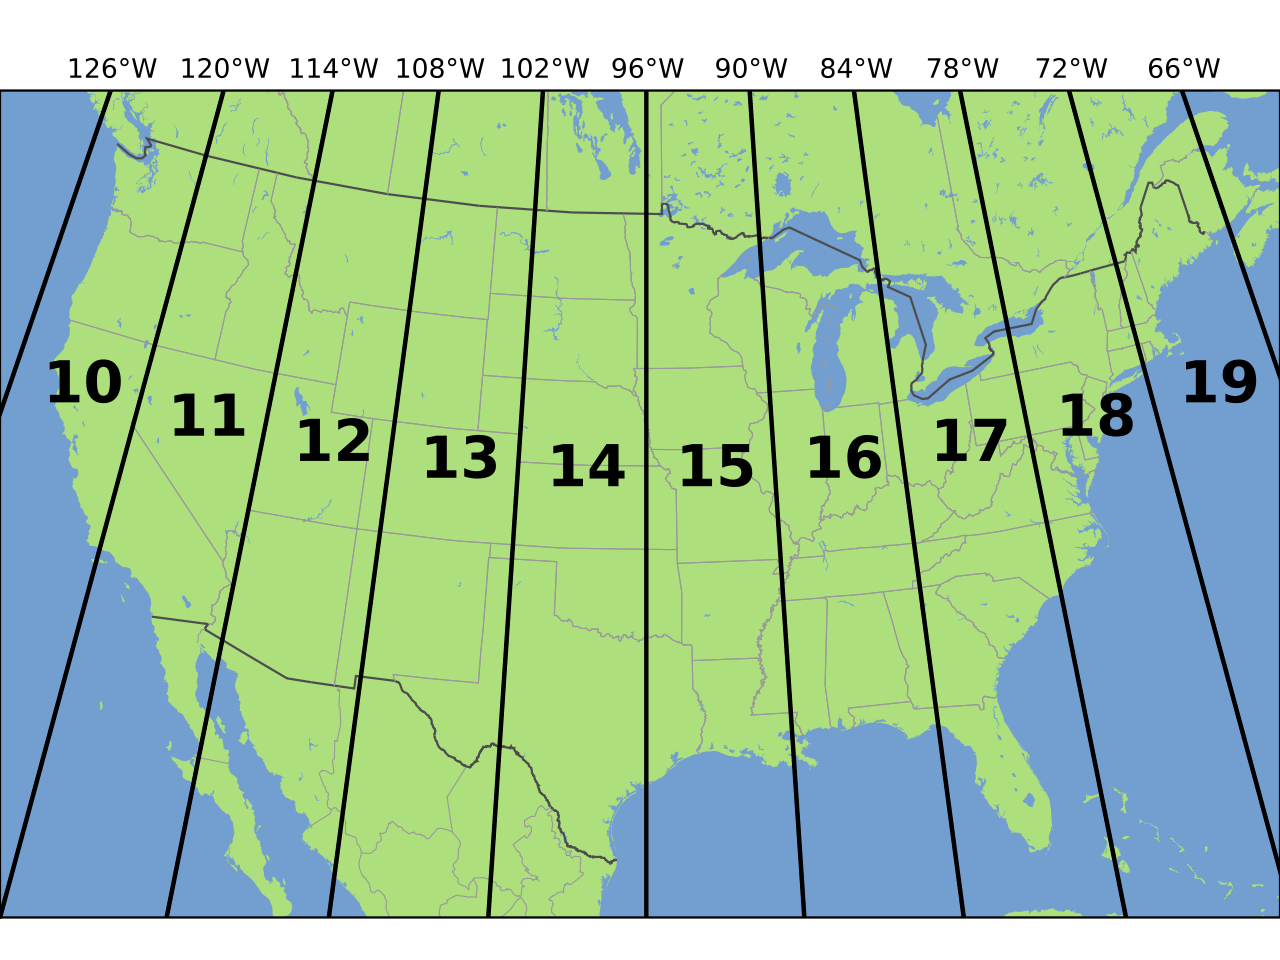
\includegraphics[width=0.3\textwidth]{Figures/UTM-zones.png}
	\caption{UTM zones across the continental United States. Source: \cite{chrismurf_2009}.
		\label{fig:utm-zones}}
\end{figure}

When working with 2D projected geographic data, we employ three basic spatial entities or primitives that can be embedded on the plane \cite{iso_simple_features}:

\begin{itemize}
	\item Points -- having a location.
	\item Lines -- comprising two or more locations in an ordered sequence.
	\item Polygons -- areas defined by three or more vertex locations in an ordered sequence.
\end{itemize}

\section{Geographic Information Systems (GIS)}

A Geographic Information System (GIS) is any system that is specifically designed to work with spatial data. GIS systems are implementations of some standard tasks, which may be present in as programming language libraries or functions, and/or as graphical user interfaces \cite{fox_spatial_2018}. Standard tasks include:

\begin{itemize}
	\item Converting datums and projections.
	\item Searching quickly for entities in particular regions.
	\item Searching quickly for entities with spatial relationships to other entities.
	\item Handling lots of data at large and small scales.
	\item Geographical data visualizations.
	\item Converting between standard spatial data file formats.
\end{itemize}

In this work, we do not use any GIS system, instead, we only use Python libraries for working with spatial data.

\section{Spatial files}

Shapefiles are a storage format for the Open Geo-spatial Consortium (OGC) definition: points, lines, and polygons. They are small collections of related files, usually stored together in a directory. The main file has a \textit{.shp} extension and stores the actual feature geometries. Other files that may appear along with it include \textit{.dbf} (associated non-spatial properties data), \textit{.shx} (indexing structure), and \textit{.prj} (datum/projection information) \cite{fox_spatial_2018}.

GeoJSON, Well-Known Text (WKT), and GraphML are alternatives for storing such data. Most GIS systems can convert between those formats.

The GraphML format is an XML-based file format for graphs. It supports a wide range of graph structures such as directed, undirected, and mixed graphs, hypergraphs, hierarchical graphs, and application-specific attributes; hence it is ideally suited for all kind of graphs.

We store our spatial data as shapefiles and our graphs as GraphML files because the latter do not have any size limit, unlike shapefiles (2 GB). Additionally, we use geo data frames (data frames with a geometry column containing points, lines or polygons) to read and manipulate shapefiles.

\section{OpenStreetMap}

For this work, we obtain our street network from OpenStreetMap (OSM) because it is free and open-source.

OSM is a collaborative worldwide mapping project that provides a free and publicly editable map of the world. In February 2021, there were over 7M registered contributors, as outlined on the OSM wiki \cite{osm-wiki}. It was created as the solution for restrictions on use or availability of map data. 

In Mexico, OSM imported the 2015 INEGI's Marco Geoestadístico Nacional (MGN) and the Red Nacional de Caminos (RNC) road data during the years 2015 and 2016 as part of the two OSM projects: Mexico Main Road Network Import Project \cite{osm_RNC_project}, and Mexico's Administrative Divisions Import Project \cite{osm_MGN_project}. Additionally, individual contributions have been made from OSM members to keep updated and accurate the data.
Acquiring the spatial data from OSM is made via an API, called Overpass, to retrieve any data in the database. However, its usage and syntax are somewhat difficult and there are other services available that can simplify the process.

OSMnx is a Python library that overrides the difficult usage of OSM APIs (see subsection \ref{subsection:osmnx}). For the purpose of this work, we download the drivable public streets, but other types can also be downloaded if available: drivable public streets with service roads, pedestrian roads, and cycling roads.

\section{Network Analysis Tools}


All the tools here presented are Python language packages or libraries. Python was chosen because it is a popular language, free, open-source, easy for beginners, powerful, and it gives us the ability to work interactively and easy integration with other Python libraries.


\subsection{NetworkX}

NetworkX is a free, open-source Python language package for the creation, manipulation, and study of the structure, dynamics, and functions of complex networks \cite{hagberg-schult-swart-networkx_2008, networkx_doc}. It provides data structures for graphs, digraphs, and multigraph, and implementations of many of the algorithms used in network science. These algorithms are implemented for structure and analysis measures, such as shortest paths, betweenness centrality, clustering, degree distribution and many more.

In addition NetworkX can read and write various graphs formats (e.g., adjacency list, edge list, GEXF, GML, pickle, GraphML, JSON, LEDA, YAML, SparseGraph6, Pajek, and GIS Shapefile), and provides generators for classic graphs, random graphs, and synthetic networks.

We use NetworkX for graph manipulation and analysis. Its modules are easy to use and it is well-documented. Furthermore, OSMnx uses NetworkX under the hood.

\subsection{GeoPandas}

Python's spatial data frame library is called GeoPandas \cite{geopandas}. GeoPandas is an open source project that allows easier manipulation of geospatial data. It extends the datatypes used by pandas (data series and data frames) \cite{pandas, mckinney-proc-scipy-2010} to allow spatial operations on geometric types (points, lines, polygons). It uses shapely for geometric operations \cite{shapely}, fiona for spatial data file access \cite{fiona}, as well as descartes \cite{descartes} and matplotlib \cite{matplotlib, Hunter:2007} for plotting.

We use GeoPandas for manipulate, visualize, read and save spatial and socio-demographic data. 

\subsection{OSMnx}
\label{subsection:osmnx}

OSMnx \cite{boeing_osmnx_2017} is a free, open-source Python package to download spatial data from OpenStreetMap and model, project, visualize, and analyze real-world street networks (e.g., walking, driving, or biking network) including node elevations and street grades. It also allow us to save the street network as shapefiles, GeoPackages, and GraphML files for later use.

OSMnx is built on top of GeoPandas, NetworkX, and matplotlib and interacts with OpenStreetMap's APIs. Thanks to that we can conduct topological and spatial analyses that OSMnx automatizes for calculating dozens of indicators, as well as calculating and visualizing the street network, street bearings and orientations, shortest-path routes.

\subsection{PySAL}

Python Spatial Analysis Library (PySAL) is an open-source, cross-platform library for geospatial data science and spatial analysis \cite{pysal2007}.

PySAL is a family of packages and is divided into four components:

\begin{itemize}
	\item Explore -- It includes modules to conduct exploratory analysis of spatial and spatio-temporal data, focused on enabling better understanding of patterns in the data.
	\item Model -- It focuses on confirmatory analysis to model spatial relationships in data with a variety of models.
	\item Viz -- It supports the creation of geovisualizations and visual representations of outputs from a variety of spatial analyses. 
	\item Lib -- It help us to solve a wide variety of computational geometry problems including graph construction from polygonal lattices, lines, and points, construction and interactive editing of spatial weights matrices and graphs, computation of spatial relationships, and reading and writing of spatial vector data.
\end{itemize}

From this tool, we used the lib component to construct the connectivity matrix of AGEBs for the clustering algorithm.

\section{Related work}

Spatial networks have been subject of study in many forms through the years. These forms, such as locations, flows of people and goods, activities, etc. are commonly studied involving time and space to make and answer questions in the complex system field to discuss the importance and evolution of networks.

Barthélemy's work \cite{barthelemy_spatial_2011, barthelemy_2018} provides an important, comprehensive review of spatial networks properties, models and measures for their analysis. The information presented in his work explains in very detail the constraints and effects of spatial networks in complex systems and its processes.

Other authors have tried to contribute by complementing the work made by Barthélemy. O'Sullivan \cite{osullivan2014} describes some important concepts and definitions placing particular emphasis on high-level structure in networks. On the other hand, Anderson \cite{anderson_2020} evaluates the integration of geographic information systems (GIS) and complex spatial networks to explore the development and applications of geographic automata systems (GAS), which are network-based automata models.

In recent years, Geoff Boeing has made relevant contributions to the field of spatial network analysis, specifically for street networks. He has developed a tool previously mentioned in this work: OSMnx \cite{boeing_osmnx_2017}. With such tool, he has done multiple studies regarding the analysis of urban street networks \cite{Boeing2019-morphology}. From developing two new indicators (spatial planarity ratio, and the edge length ratio) for measuring planarity and describing infrastructure and urbanization \cite{boeing2020-planarity} to analyzing and comparing thousands of urban street networks \cite{boeing_multi-scale_2018}  and exploring patterns and configuration through visualization methods \cite{Boeing2020-urban-form-osm}.

%%% Local Variables:
%%% mode: latex
%%% TeX-master: "../upyreportmain"
%%% End:

\chapter{Methodology and development}
\label{cha:chapter3}

\added[id=GP]{In this Chapter, I provide a description of the workflow followed during the analysis of the road network.}

\replaced{Most of the analysis}{This work} was done using Jupyter notebooks, \added{an open format which allows for documented and reproducible workflows.} \added{. All notebooks are stored in} a GitHub repository (\url{https://github.com/gperaza/road-network}\added{, private at the time of writing, since it still contains preliminary work.}). \replaced{The}{This} repository's root contains an environment definition file and a notebooks folder. Within that folder, the repository contains \added{nested subfolders, }one folder for the work done in Mérida, Yucatán, and other folder for the different cities in México, that are beyond the scope of this report. The following notebooks \added{(which included the analysis reported here)} are included in the Mérida folder:

\begin{enumerate}
\item Data preparation: downloading/modeling and calculating network stats of Mérida's road network and its urban AGEBs.
\item Analysis of the road network of Mérida and its urban AGEBs.
\item Cluster analysis of the urban AGEBs.
\end{enumerate}

To \replaced{reproduce the analysis}{run the code examples} in this resource repository, we simply \replaced{execute each notebook}{run everything} in a pre-built Anaconda environment. This process is detailed in the following section.

\section{The Environment}

\replaced{The}{This} project's repository contains an Anaconda environment file in \verb|yaml| format\deleted{(i.e., .yml)} for running the Jupyter notebooks on any computer. Anaconda \cite{anaconda} is a data science platform that facilitates package management and deployment. It is available for Windows, Linux and macOS. We use the Individual Edition, which is the open-source distribution of Anaconda.

First, download and install Anaconda Individual Edition. Once it is installed and running on your computer, run the following code in the terminal window:

\begin{lstlisting}[language=bash]
$ conda config --add channels conda-forge
$ conda env create --file road-network-project.yml
$ conda activate road-network-project
$ jupyter lab
\end{lstlisting}

Loading the configuration file ensures all appropriate packages are loaded with the required versions. This avoids dependency problems among packages, which are hard to resolve by hand.

With the environment active, it is possible to access and edit the notebook files from the Jupyter Lab interface, which is available though a web browser at \url{http://localhost:8888}.

\section{Data Collection}

This work uses OSMnx to download the street network of Mérida and its AGEBs \added{from Open Street Map}. The road network is loaded into a graph model (using NetworkX), corrected, and analyzed. OSMnx also allows for visualization at municipal and neighborhood (AGEB) scales.

To obtain the street network, we define a function to download and save the graph of the municipality, or, if already present, load it from a previously stored NetworkX graph object:

\begin{lstlisting}[language=Python]
def get_roads_osmnx(places, update=False, proj=False, crs=None):

    dirpath = pathlib.Path('./data/networks/')
    filepath = dirpath/'merida-road.graphml'
    logpath = dirpath/'log'

    if filepath.exists() and not update:
        G = ox.load_graphml(filepath)
    else:
         # get drivable public streets network,
         # aka road network, without service roads,
         # e.g. private, parking lots, etc.
         # use retain_all if you want to keep all
         # disconnected subgraphs (e.g. when your
         # places aren't adjacent)
        G = ox.graph_from_place(places, network_type='drive')
        ox.save_graphml(G, filepath=filepath, gephi=False)

    if proj:
        G = ox.project_graph(G, to_crs=crs)

    print(f"Graph created at: {G.graph['created_date']}")
    return G, *ox.graph_to_gdfs(G)

places = [{'county' : 'Merida', 'state' : 'Yucatan', 'country' : 'Mexico'}]
G_proj, nodes_proj, edges_proj = get_roads_osmnx(places, update=False,
                                                 proj=True, crs=3857)
\end{lstlisting}

OSMnx geocodes the query "Merida, Yucatan, Mexico" to retrieve the place boundaries of that city from the Nominatim API. It then retrieves the drivable street network data within those boundaries from the Overpass API and constructs a graph model (via NetworkX). OSMnx simplifies/corrects the network topology in such way that nodes represent intersections and dead-ends, and edges represent the street segments linking them. Finally, the functions saves the constructed graph as a GraphML file as to not download the same data again.

Note that the graph is projected to the WGS84 Pseudo-Mercator CRS ("EPSG:3857"). We do not use the commonly used CRS WGS84 latitude-longitude projection ("EPSG:4326"), since in such CRS the coordinates are given in degree units, and we required meters for distance calculations. For that reason, we use the "EPSG:3857" projection, where coordinates are given in meters. This last projection is the one that Google, OpenStreetMap, Bing, ArcGIS, ESRI, etc. use for rendering their maps~\cite{epsg3857}.

\comment[id=GP]{I thought we were using an UTM projection? What happened?}

Besides the graph object, the function, also returns node and edge GeoDataFrames, used for tabular storage and analysis of such entities. This is possible since OSMnx models all networks as NetworkX MultiDiGraph objects and allows conversion among different network models and data structures, i.e., from and to:

\begin{itemize}
 \item Undirected MultiGraphs.
 \item DiGraphs without (possible) parallel edges.
 \item GeoPandas node/edge GeoDataFrames.
\end{itemize}

\comment[id=GP]{If AGEBS are note previously defined we need to define them before the following paragrah. I see you defined them in a couple paragraphs below, you need to move that definition here with a short discussion of why we are using agebs.}

We collected information for Mérida's urban AGEBs from the Institute of Statistics and Geography's (INEGI) National Geoestatistical Framework (MG, by the acronym in spanish) and from socio-demographic data from INEGI's 2020 Population and Housing Census (2020 Census) conducted from March 2 to March 27, 2020~\cite{2020census}.

The MG is a mexican unique national system designed by INEGI to correctly reference statistical information from censuses and surveys with the corresponding geographic locations \cite{manualMGN}. It is conformed by geostatistical areas divided into three dissaggregation areas (see Figure \ref{fig:MGN_divisions}):

\begin{itemize}
 \item State geoestatistical areas (AGEE).
 \item Municipal geoestatistical areas (AGEM).
 \item Basic geoestatistical areas (AGEB).
  \begin{itemize}
   \item Rural AGEB.
   \item Urban AGEB.
  \end{itemize}
\end{itemize}

\begin{figure}[htpb]
  \centering
  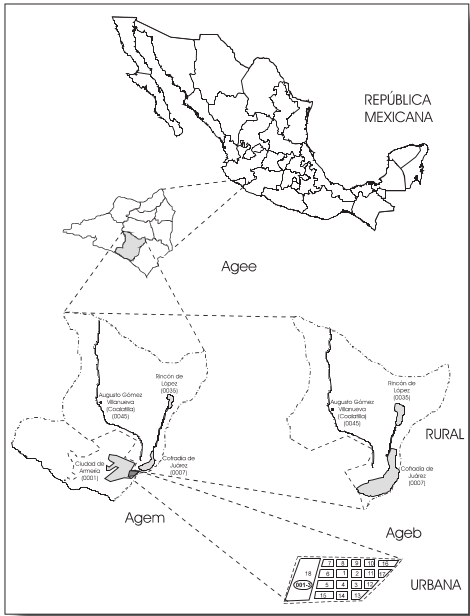
\includegraphics[width=0.6\textwidth]{Figures/MGN_divisions.png}
  \caption{MG dissaggregation areas. Retrieved from: \cite{manualMGN}.
    \label{fig:MGN_divisions}}
\end{figure}

Urban AGEBs are the geographic area, subdivision of municipal areas, occupied by a set of blocks, generally ranging from 1 to 50, perfectly delimited by streets, avenues, walkways or any other easily identifiable feature on the ground and whose land use is mainly residential, industrial, services, commercial, etc., only assigned within urban localities (see Figure \ref{fig:ageb_division}).

\begin{figure}[htpb]
  \centering
  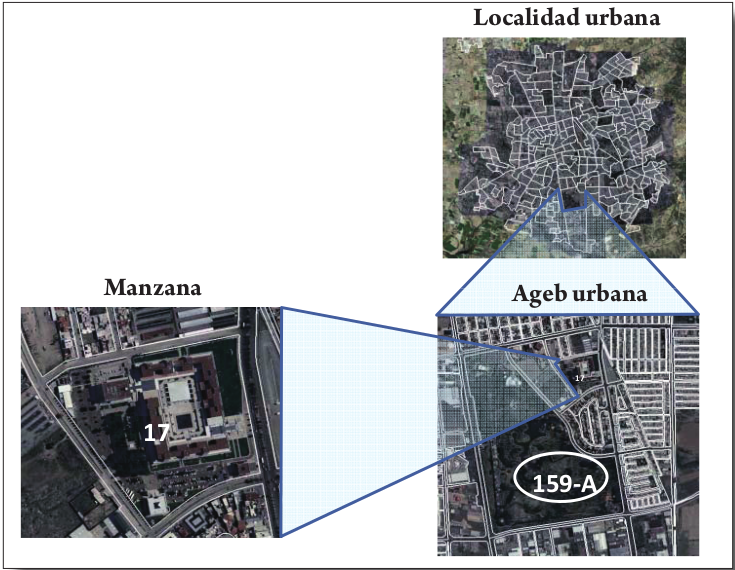
\includegraphics[width=0.7\textwidth]{Figures/ageb_division.png}
  \caption{Urban AGEB dissaggregation areas. Retrieved from: \cite{manualMGN}.
    \label{fig:ageb_division}}
\end{figure}

The MG data (downloaded at~\cite{MG_data}) contains shapefiles for every dissaggregated area of every mexican state. It is made up of 32 folders, each one named by the geoestatistical key of the federal entity (from 1 to 32), with a national total of 2,469 municipal geoestatistical areas, 45,397 polygons of rural localities, and 4,911 polygons of urban localities, 295,779 points of rural localities, 350 polygons of island territory, 17,469 basic rural geostatistical areas, 63,982 basic urban geostatistical areas and 2,513,853 urban and rural blocks (including scattered hamlets). The information maintains associated names and geostatistical keys as attributes.

The MG references every dissaggregated area with a unique numeric key. The structure of such geostatistical key is represented in Figure~\ref{fig:key_structure}.

\begin{figure}[htpb]
  \centering
  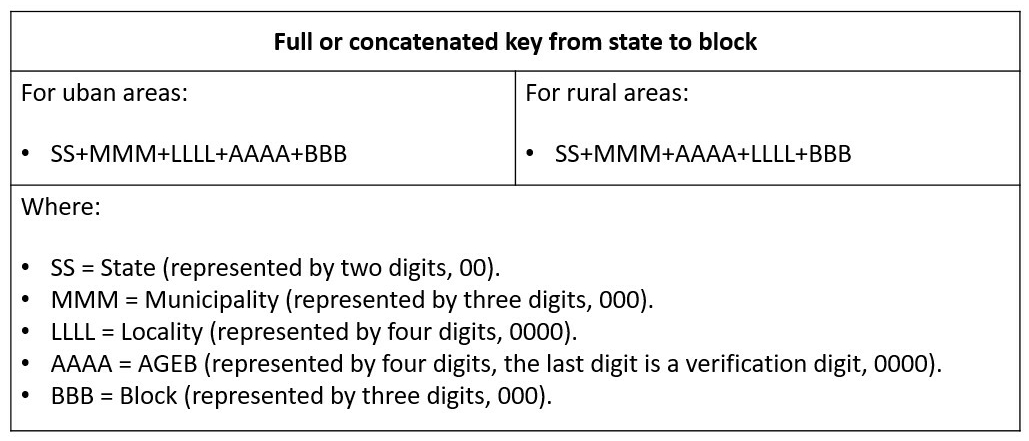
\includegraphics[width=0.8\textwidth]{Figures/key_structure.jpg}
  \caption{MG's geostatistical key structure. Retrieved from: \cite{manualMGN}.
    \label{fig:key_structure}}
\end{figure}

Every state folder of the MG is composed of three subfolders:
\begin{itemize}
\item Catalogs (catálogos): contains the product catalogs and documentation.
\item Data set (conjunto\_de\_datos): contains 32 folders, each one corresponding to the state geoestatistical key.
\item Metadata (metadatos): contains 32 files, each one with the corresponding state geostatistical key, in xml and txt format, and a generic metadata with national information.
\end{itemize}

The file names are formed with the state geoestatistical key and the following suffixes of the file content:

Where \textbf{ee} corresponds to the state geoestatistical key (from 01 to 32).

\begin{table*}[htpb]
  \centering
  \label{tab:MG_filenames}
  \footnotesize
  \begin{tabular}{ l l }
    ee\textbf{ent} & State geoestatistical areas \\
    ee\textbf{mun} & Municipal geoestatistical areas \\
    ee\textbf{ar} & Basic rural geoestatistical areas \\
    ee\textbf{l} & Polygon of urban and rural localities \\
    ee\textbf{lpr} & Rural point locations \\
    ee\textbf{ti} & Island territory\\
    ee\textbf{a} & Basic urban geoestatistical areas \\
    ee\textbf{m} & Block polygons\\
    ee\textbf{fm} & Block fronts \\
    ee\textbf{e} & Road axes \\
    ee\textbf{cd} & Scattered hamlet \\
    ee\textbf{sia} & Complementary area-type services and information (green areas, medians, traffic circles) \\
    ee\textbf{sil} & Complementary line-type services and information
                     (rivers, railroads, streams) \\
    ee\textbf{sip} & Complementary point-type services and information
                     (municipal palaces, parks or gardens, etc.) \\
    ee\textbf{pe} & External polygon \\
    ee\textbf{pem} & External polygon of blocks \\
  \end{tabular}
\end{table*}

Layers with suffix \textbf{ti}, \textbf{cd}, \textbf{pe}, \textbf{pem}, \textbf{sia}, \textbf{sil}, \textbf{sip}, are included only if the locality has this type of information.

INEGI's 2020 census data was downloaded from~\cite{2020census} as a CSV file per state with main results by AGEB and urban block (option eligible on the portal). In this work, we use only MG and census data for Yucatán (folder \verb|31_yucatan| from the MG and file \verb|31a.shp| of the basic urban geoestatistical areas).

\section{Data Exploration and Preparation}

Mérida's street network has 93485 edges and 35105 nodes, and covers a convex hull area of 1,032.4 km$^2$ that comprises the 874.4 km$^2$ of the Mérida municipality's area \cite{2020census}. However, the network is disconnected due to unfinished roads or roads at the boundary. Thus, we retain only the largest connected component (see Figure \ref{fig:merida-street-network}), which has 93371 edges and 35031 nodes, comprising the 99.9\% of edges and 99.8\% of nodes from the whole network. The covered area is the same. Figure \ref{fig:merida-street-network-boundary} shows the street network within the municipal boundary of Mérida.

\begin{figure}[htpb]
  \centering
  \includegraphics[width=0.5\textwidth]{Figures/merida-road-network.png}
  \caption{Mérida municipality street network.
    \label{fig:merida-street-network}}
\end{figure}

\begin{figure}[htpb]
  \centering
  \includegraphics[width=0.5\textwidth]{Figures/merida-road-network-boundary.png}
  \caption{Mérida municipality street network with municipal boundary.
    \label{fig:merida-street-network-boundary}}
\end{figure}

\replaced{As encoded by OSMnx,}{If we look at the node and edge attributes of the network, we see that} nodes are indexed by an integer value (the ID from OSM) and posses several features: $x$ and $y$ coordinates, number of streets intersecting the node (street count), type of intersection, latitude and longitude. \replaced{There are a total of}{We have} 773 nodes that are labeled by their intersection type, such as crossing, mini roundabout, motorway junction, traffic signals, turning circle, or turning loop. \deleted{Remember that nodes are considered street intersections.}

Edges (roads) and are indexed by \added(a tuple with three values): their starting and ending nodes, \replaced{and an edge key}{and a zero}. \deleted{They are tuple objects.} As mentioned, the third integer is the edge key, since in a multigraph we can have potentially more than one edge between the same pair of nodes. Each edge is identified by an integer key, and is often zero in Merida's road network, since multi edges are rare. Other edge attributes include: the ID from OSM, type of road (e.g., primary, primary link, secondary, secondary link, tertiary, tertiary link, trunk, trunk link, residential, living street, and unclassified), maximum speed, length of the road, name of the street, width, and whether it is a lane, bridge, junction, tunnel, or access road. We have 19842 lane roads, 56 bridges, 1366 road junctions, 2 tunnel roads, and 5 access roads.

One of the main objectives of the project is to analyze how street network metrics change with scale. As a first step, we imported AGEBs from the MG to create a subgraph for each different AGEB. Additionally, to include socio-demographic data in the analysis, we merged both MG and 2020 Census data, since the census dataset does not include the polygons of the AGEBs. The merging process is described in the following.

The 2020 Census data contains missing information recorded as * (asterisk) or N/D (Not Available). We replaced such values with zero (0). After,  we manually set the data types of each feature from string to the true type (float), according to~\cite{census_data}. We also dropped totals by municipality and locality as only totals by AGEB are processed in the analysis.

We create a new column in the 2020 Census dataframe to store the (full) geostatistical key, built by combining values from the geostatistical keys of state, municipality, locality, and AGEB, while omitting block information.
\comment[id=GP]{What are blocks? I think the rest of the paragraph is unecesarly descriptive. This are mostly standard preprocessing steps that, if needed, can be look up in the notebooks. Just mention you drop redundat columns and perform an inner merge.}
 We add missing zeros to the values of the municipality and locality geostatistical key to fulfill the appropiate length. Also, we change the data types of the state, municipality, and locality geostatistical keys from integer to string to concatenate them. Next, we drop columns from the 2020 Census dataframe that will be duplicated after the merging. Finally, we perform the merge with the MG dataframe on the concatenated geostatistical key column present in both dataframes using the inner merge type that uses the intersection of columns from both dataframes, similar to a SQL inner join~\cite{pandas_merge}.

The MG has geometric data from 1532 AGEBs, while the 2020 Census has data from 1432 AGEBs for Yucatán. After the merge, we ended up with the subset of 1432 AGEBs in both data sets. We further narrow the selection to include only the 523 urban AGEBs belonging to the city of Mérida. The merged geodataframe was saved as shapefiles under the name \verb|merida\_ageb\_census\_data.shp| projected in the Pseudo-Mercator CRS.

Next, we created a subgraph for each AGEB, containing only the portion of the network within each AGEB. To do this, we first created a new column with each AGEB cover area, in meters, calculated from each AGEB's polygon. The dataframe is re-project into the Mercator projection, which is the projection expected by OSMnx. Then, we create queries from the AGEBs geodataframe to automate the downloading and saving of each AGEB's road network. The queries contain the path where graphs will be saved, the polygon of the AGEB to be downloaded, and the area in meters of the AGEB. Every graph is saved in both shapefile and GraphML format. We ended up with 517 AGEBs specific graphs, because some AGEBs did not contain any node or edge within the requested polygon. The generation of the subgraphs takes around 32 minutes.

OSMnx includes two modules (basic and extended stats) for calculating geometric and topological network measures for street network analysis. The list of the measures is the following:

\begin{itemize}
\item Number of nodes.
\item Number of edges.
\item Average node degree.
\item Number of intersections: nodes with $>$1 physical streets connected to them.
\item Average streets per node: how many physical streets (edges in the undirected representation of the graph) connect to each node (i.e., intersection or dead-end) on average.
\item Streets per node count: number of physical streets connecting to a node.
\item Streets per node proportion: same as previous but proportion of the total, rather than counts.
\item Total edge length: sum of all edge lengths in graph, in meters.
\item Average edge length: mean edge length in the graph, in meters.
\item Total street length: sum of all edges in the undirected representation of the graph.
\item Average street length: mean edge length in the undirected representation of the graph, in meters.
\item Street segments count: number of edges in the undirected representation of the graph.
\item Node density: number of nodes divided by area in km$^2$.
\item Intersection density: intersection count divided by area in km$^2$.
\item Edge density: Total edge length divided by area in km$^2$.
\item Street density: Total street length divided by area in km$^2$.
\item Average circuity: Total edge length divided by the sum of the great circle distances between the nodes of each edge.
\item Self-loop proportion: proportion of edges that have a single node as its endpoints (i.e., the edge links nodes u and v, and u==v).
\item Clean intersection count: number of intersections in street network, merging complex ones into single points.
\item Clean intersection density: clean intersection count divided by area in km$^2$.
\item Average neighbor degree.
\item Average neighbor degree average.
\item Average weighted neighbor degree.
\item Average weighted neighbor degree average.
\item Degree centrality.
\item Average degree centrality.
\item Clustering coefficient.
\item Average clustering coefficient.
\item Weighted clustering coefficient.
\item Average weighted clustering coefficient.
\item PageRank.
\item Maximum PageRank node.
\item Maximum Pagerank.
\item Minimum PageRank node.
\item Minimum PageRank.
\item Node connectivity.
\item Average node connectivity.
\item Edge connectivity.
\item Eccentricity.
\item Diameter.
\item Radius.
\item Center.
\item Periphery.
\item Closeness centrality.
\item Average closeness centrality.
\item Betweenness centrality.
\item Average betweenness centrality.
\end{itemize}

We calculate the listed metrics for the Mérida municipality street network, except for node and edge connectivity, eccentricity, diameter, radius, center, and periphery due to exhaustion of the computer memory. The calculations lasted around 6 hours and 7 minutes. We saved the calculations in a csv file to avoid recalculation.

For each individual subgraphs AGEBs, we do not exclude any listed metric. Such calculations lasted around 47 minutes for all AGEBs. However, two AGEBs were excluded because they had only one node. Also, when we updated the local degree, betweenness and closeness centrality to global, other two AGEBs were excluded as Mérida's street network did not include any node of such AGEBs. For such reason, we ended up working with 513 AGEBs in this work (see Figure \ref{fig:merida-ageb-street-network}). Finally, we merge the network calculations with the 2020 Census and MG data into a single geodataframe, and a column for population density was added. The data was saved in shapefiles named \textit{merida\_ageb\_stats\_census.shp}.

\begin{figure}[htpb]
  \centering
 \includegraphics[width=0.5\textwidth]{Figures/merida-ageb-road-network.png}
  \caption{Mérida street network with urban AGEBs.
    \label{fig:merida-ageb-street-network}}
\end{figure}

\section{Data Modeling}

As one of our objectives is to perform a clustering algorithm on the AGEBs to find similar AGEBs based on socio-demographic data and their network measures, we must choose how our AGEBs are going to be interconnected.

Spatial weights are used to represent geographical relationships between two spatial observations. We consider two different approaches to construct spatial weights based on contiguity/adjacency relations. Such approaches arises from the legal moves that different chess pieces can make. Rook contiguity considers two polygons as connected if they share an edge on their border (see Figure \ref{fig:rook-contiguity}). But Queen contiguity connects two polygons if they share a one or more points on their border (see Figure \ref{fig:queen-contiguity}). As result, queen representation has more neighbors than rook has. We chose a rook representation as it exploits the sparse nature of contiguity weights matrices \cite{rey_geo_ds_2020}.

\begin{figure}[htpb]
  \centering
  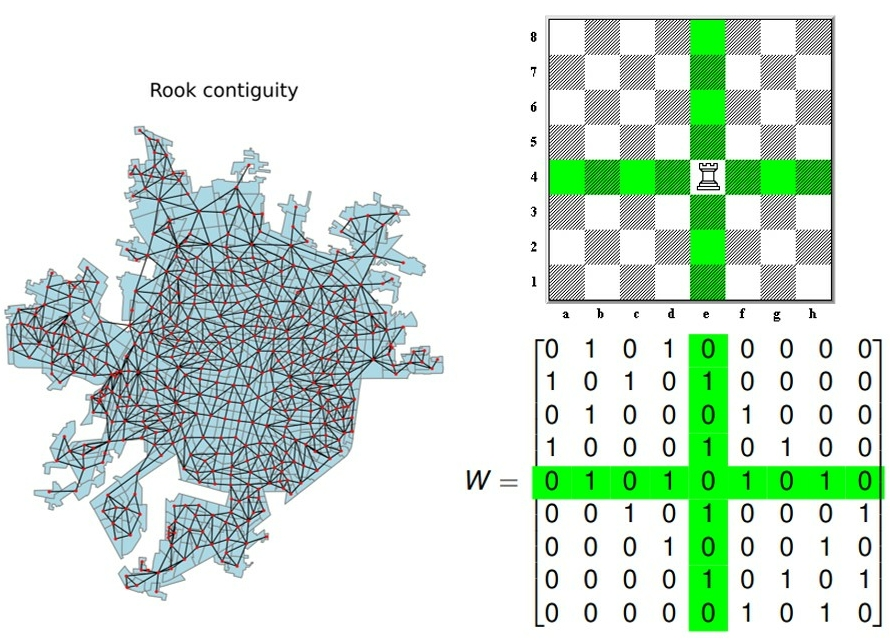
\includegraphics[width=0.8\textwidth]{Figures/rook-contiguity.jpg}
  \caption{Rook contiguity.
    \label{fig:rook-contiguity}}
\end{figure}

\begin{figure}[htpb]
  \centering
  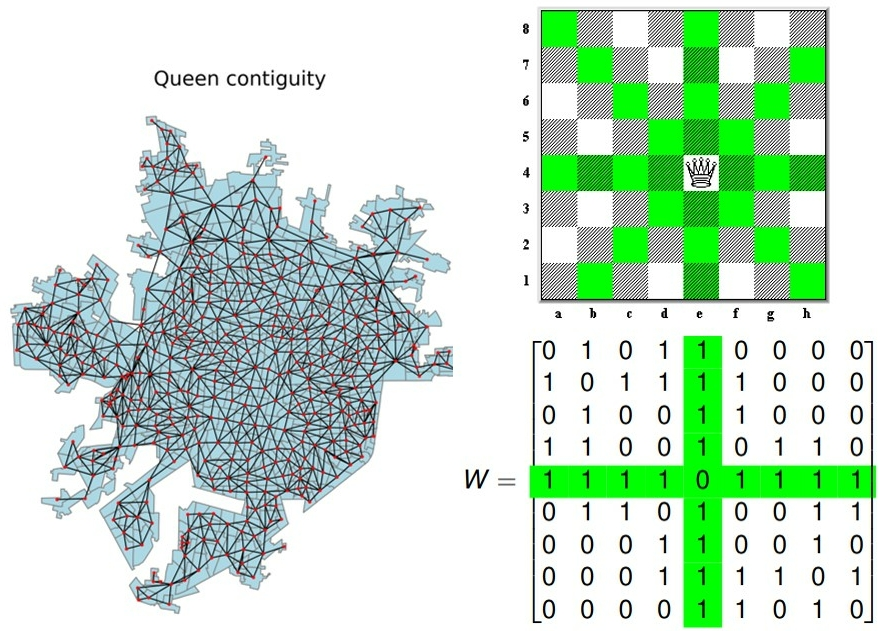
\includegraphics[width=0.8\textwidth]{Figures/queen-contiguity.jpg}
  \caption{Queen contiguity.
    \label{fig:queen-contiguity}}
\end{figure}

When we construct the rook adjacency matrix, we had to eliminate some AGEBs that were disconnected (islands). We drop AGEBs from Mérida localities such as San José Tzal, Komchen, Chablekal, as well as the Military Base and the Airport of Mérida. The adjacency matrix is used to add connectivity constraints to the clustering algorithm to impose a certain structure defining for each sample the neighboring samples. Also, it makes the algorithm faster.

The clustering algorithm that we use in this work is the hierarchical clustering (also known as connectivity-based clustering) that builds nested clusters by merging or splitting them recursively. The hierarchy of clusters is represented as a tree (or dendrogram). A machine learning Python library, called Scikit-Learn \cite{scikit-learn}, provides us their implementation of the agglomerative hierarchical clustering algorithm.

The agglomerative clustering is the most common type of hierarchical clustering used to group objects in clusters based on their similarity. It uses a bottom-up approach: each observation starts in its own cluster, then pairs of clusters are successively merged until all clusters have been merged together \cite{hierarchical_scikit}. The linkage criteria determines the metric used for the merge strategy:

\begin{itemize}
\item \textbf{Ward} minimizes the variance of the clusters being merged.
\item \textbf{Maximum} or \textbf{complete linkage} minimizes the maximum distance between observations of pairs of clusters.
\item \textbf{Average linkage} minimizes the average of the distances between all observations of pairs of clusters.
\item \textbf{Single linkage} minimizes the distance between the closest observations of pairs of clusters.
\end{itemize}

We select ward linkage as the most suitable because we only have an adjacency matrix, not a distance matrix.

The final step was to find the appropiate number of clusters for the algorithm. Based on empirical observation, 14 clusters were selected as they best describe similarity between AGEBs.


%%% Local Variables:
%%% mode: latex
%%% TeX-master: "../upyreportmain"
%%% End:

\chapter{Results}
\label{cha:chapter4}

\section{Municipal scale}

Table \ref{tab:measures_urban_city} presents statistics for the Mérida's municipality street network. 

Mérida has 35031 intersections and 5 million meters of linear street. It is 96\% less circuitous than straight-line edges would be. The average street segment length (a proxy for block size) is 99 meters. And it has 31 intersections per km$^2$.

\begin{table*}[htbp]
	\centering
	\caption{Selected measures of all Mérida street network.}
	\label{tab:measures_urban_city}
	\small
	\begin{tabular}{ l r }
		\toprule
		measure                                          &              \\
		\midrule
		Area (km\textsuperscript{2})                     & 1032.365       \\
		Avg of the avg neighborhood degree               & 2.843        \\
		Avg of the avg weighted neighborhood degree      & 0.045       \\
		Avg circuity                                     & 0.964 \\
		Avg clustering coefficient                       & 0.030        \\
		Avg weighted clustering coefficient              & 0.001 \\
		Intersection count                               & 31837      \\
		Avg degree centrality                            & \textless0.001          \\
		Edge density (km/km\textsuperscript{2})          & 9013.845         \\
		Avg edge length (m)                              & 99.662          \\
		Total edge length (km)                           & 9306      \\
		Proportion of dead-ends                          & 0.091          \\
		Proportion of 3-way intersections                & 0.592         \\
		Proportion of 4-way intersections                & 0.312          \\
		Intersection density (per km\textsuperscript{2}) & 30.839          \\
		$m$                                              & 93371     \\
		$n$                                              & 35031      \\
		Node density (per km\textsuperscript{2})         & 33.933         \\
		Max PageRank value                               & \textless0.001 \\
		Min PageRank value                               & \textless0.001 \\
		Self-loop proportion                             & 0.001        \\
		Street density (km/km\textsuperscript{2})        & 5259.333        \\
		Average street segment length (m)                & 99.177        \\
		Total street length (km)                         & 5430     \\
		Street segment count                             & 54746      \\
		Average streets per node                         & 3.130         \\
		\bottomrule
	\end{tabular}
\end{table*}

The distribution of node types (i.e., intersections and dead ends) provides an indicator of network connectedness. Mérida has 3.1 streets per intersection on average; 31\% of nodes are 4-way intersections, 59\% are 3-way intersections, and 9\% are dead-ends (see Figure \ref{fig:merida-node-types-distribution}).

\begin{figure}[h!]
	\centering
	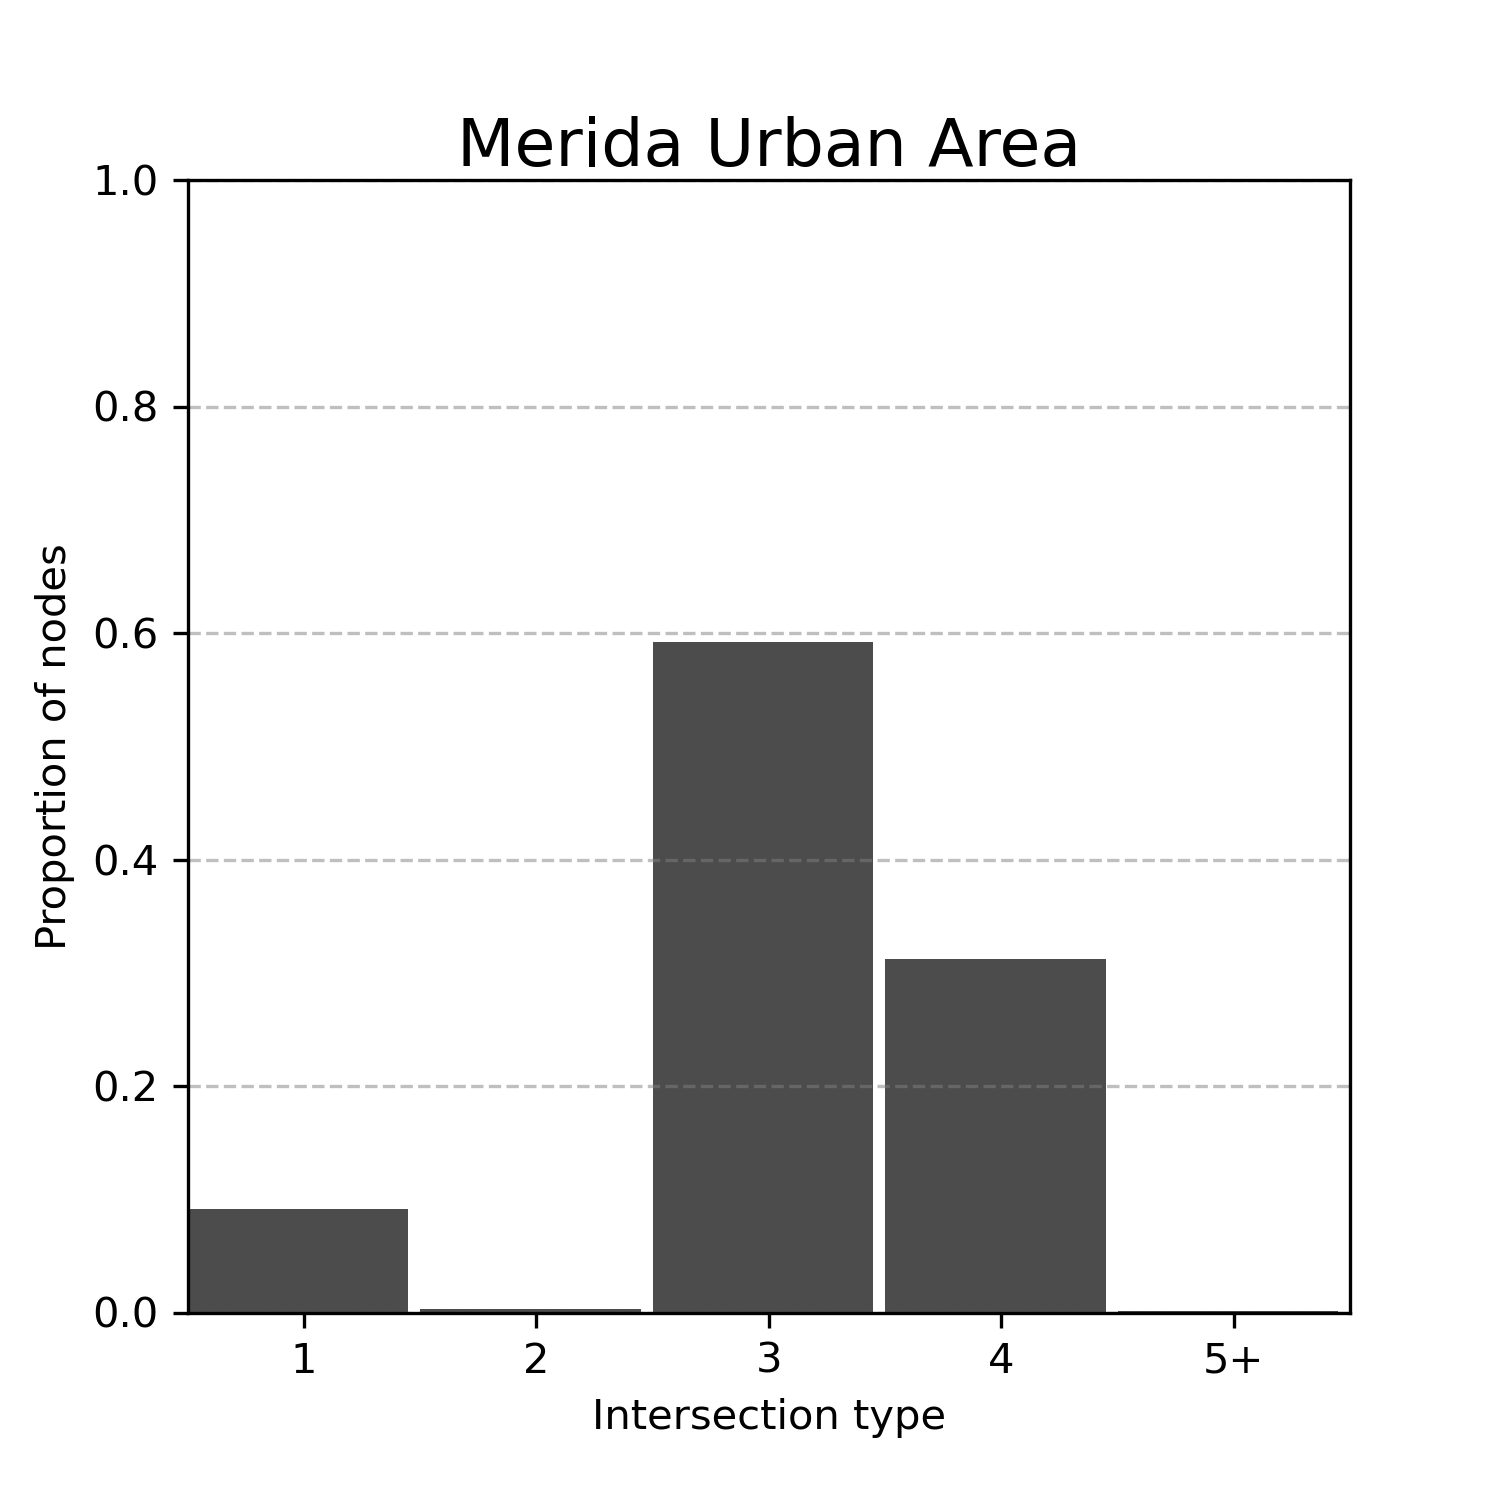
\includegraphics[width=0.5\textwidth]{Figures/merida-street-per-node-proportion-distribution.png}
	\caption{Distribution of node types in Mérida.
		\label{fig:merida-node-types-distribution}}
\end{figure}

Centrality measures identify the most important nodes in a network. We can have different ways of thinking about importance. Some of the most known centrality measures are: degree centrality, closeness centrality, betweenness centrality, and PageRank. Each of these measures gives us a different approach, or use case, to identify the most important nodes in the network \cite{menczer_fortunato_davis_2020}.

According to degree centrality, important nodes have many connections. Figure \ref{fig:merida-max-node-degree-centrality} depicts the node with highest degree centrality. This node is at the intersection of many streets that pass through it. In Figure \ref{fig:merida-degree-centrality} we can visualize all nodes by their relative degree centrality. We can observe that intersections in principal streets, avenues, and in the historical center of Mérida have low degree centrality compared to intersections in residential areas.

\begin{figure}[h!]
	\centering
	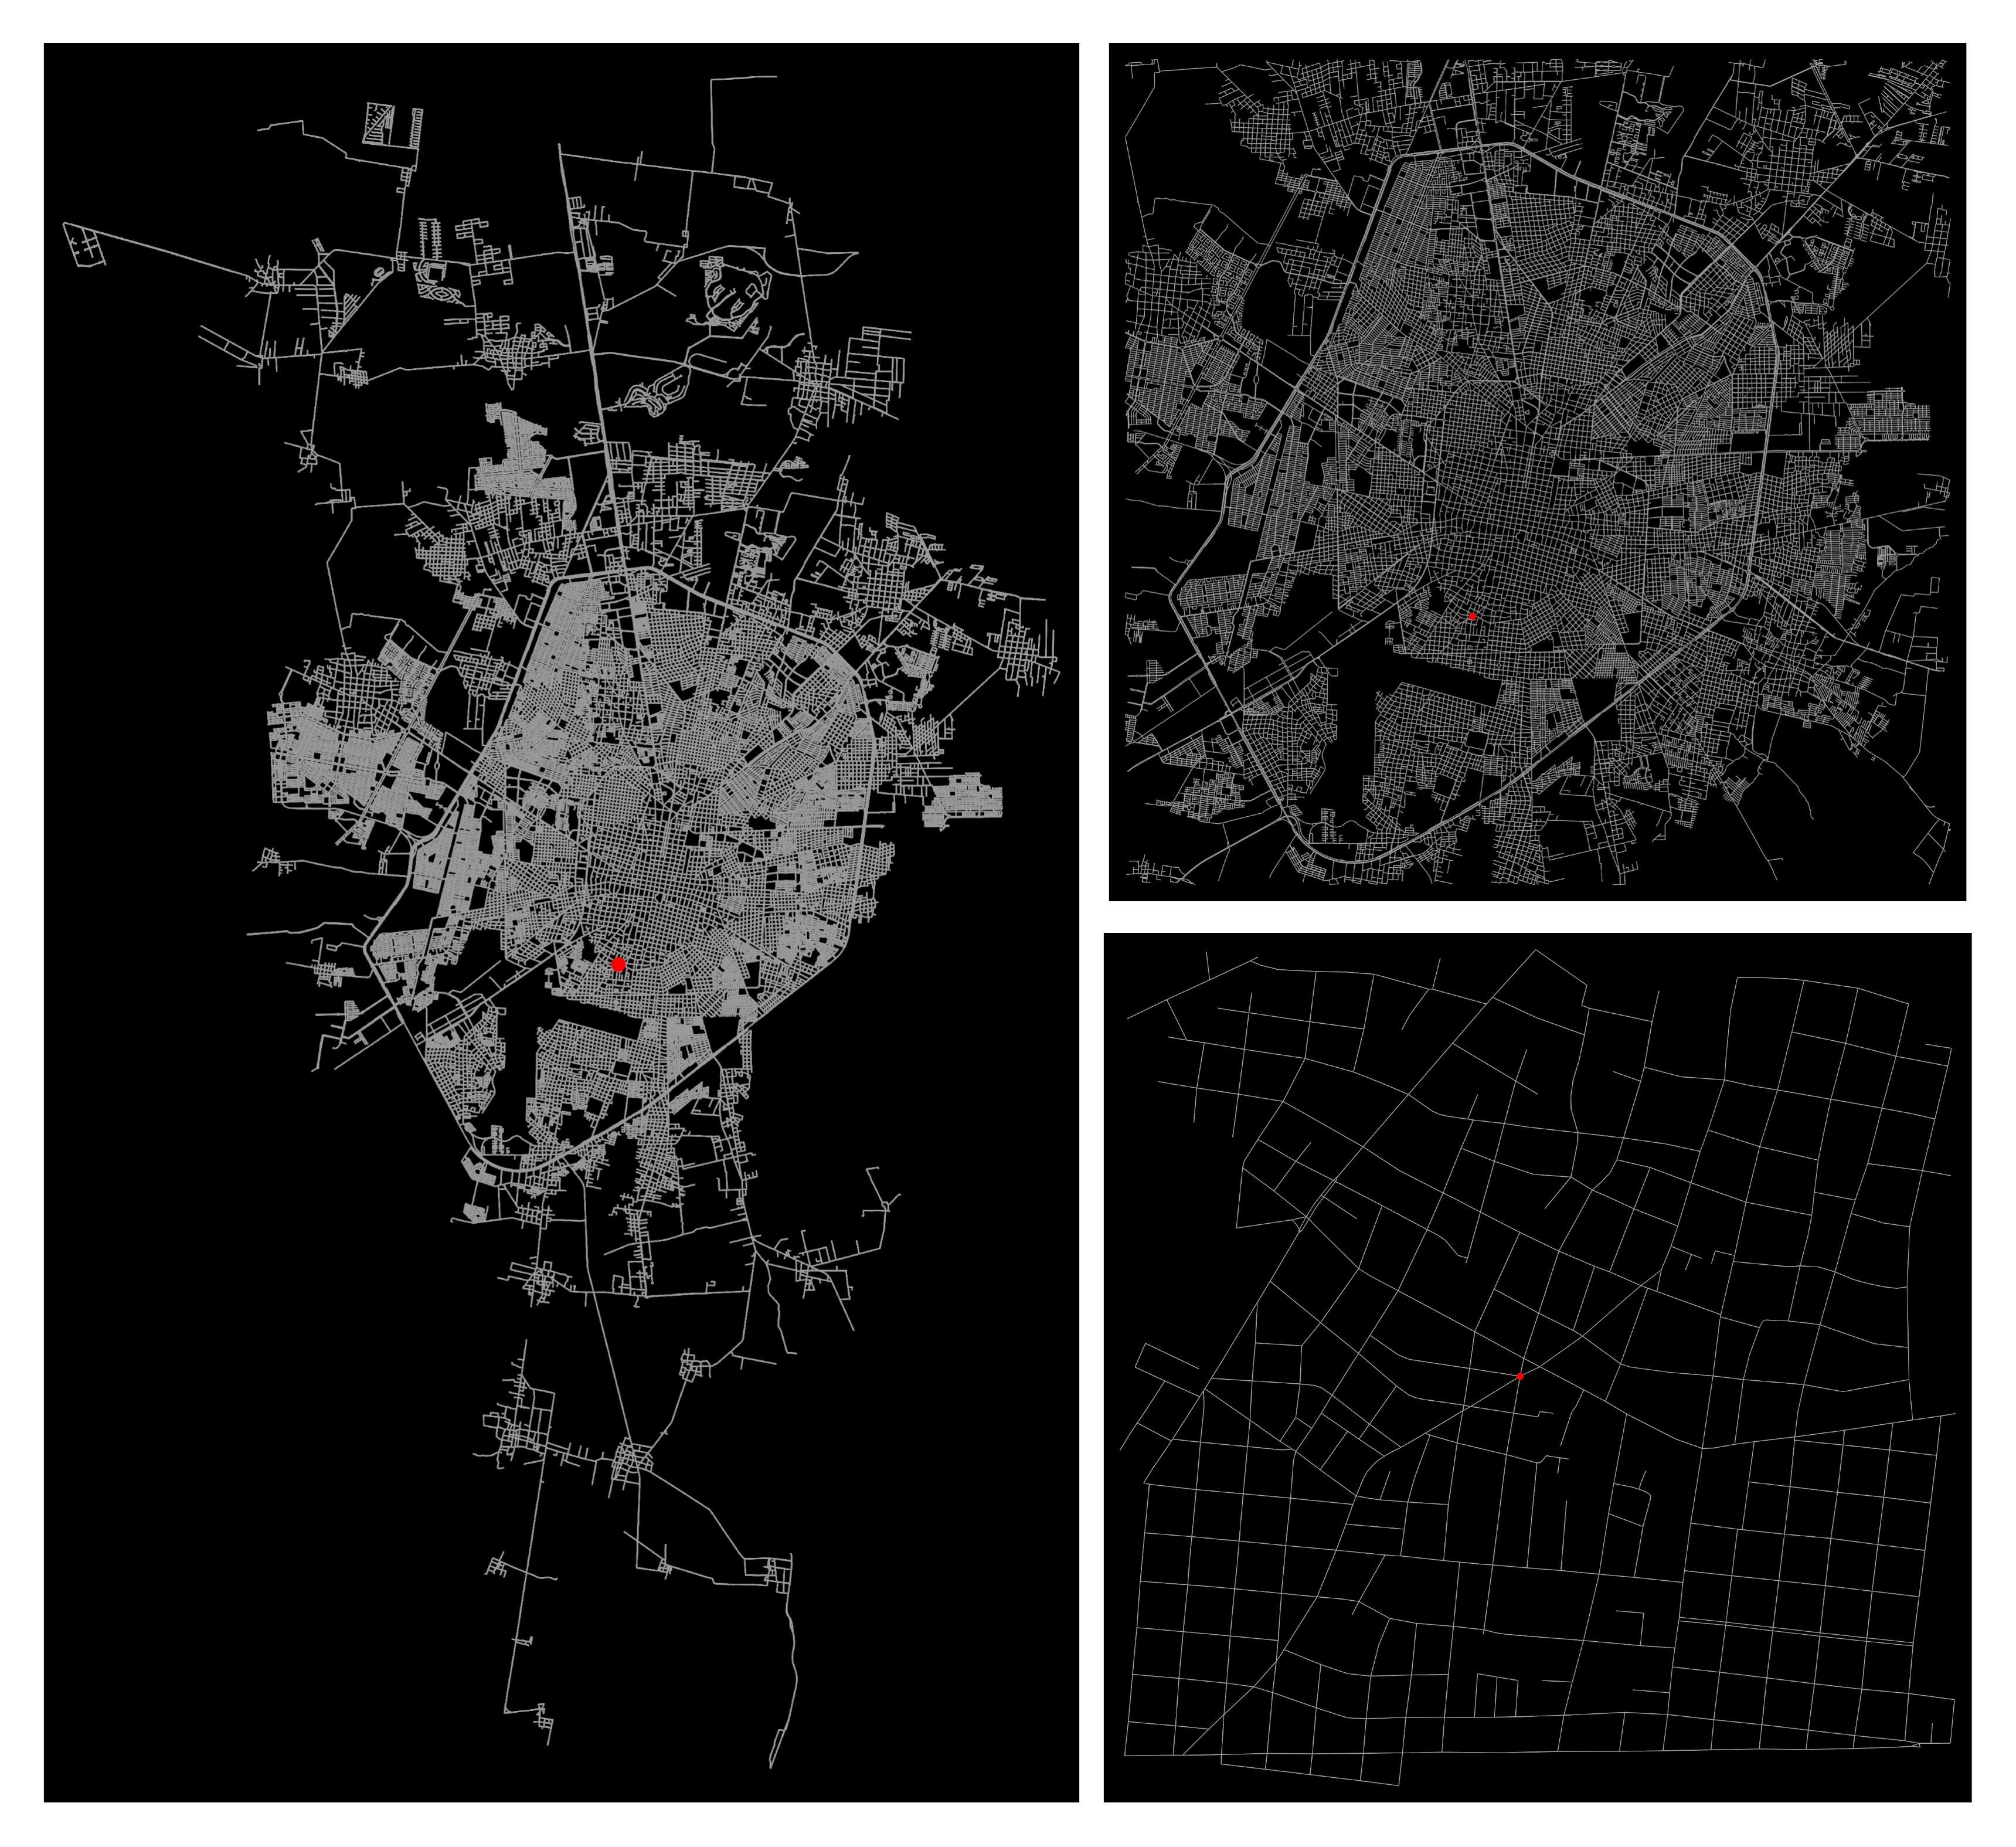
\includegraphics[width=0.8\textwidth]{Figures/merida-node-degree-centrality.png}
	\caption{Node with highest degree centrality score. The node is located at 64 street with 95 and 75 street, colonia Meliton Salazar.
		\label{fig:merida-max-node-degree-centrality}}
\end{figure}

\begin{figure}[h!]
	\centering
	\includegraphics[width=0.5\textwidth]{Figures/merida-degree-centrality.png}
	\caption{Degree centrality of all nodes in Mérida. Nodes are visualized from low (dark violet) to high (light yellow). The colors in colorspace are linearly mapped to the attribute values.
		\label{fig:merida-degree-centrality}}
\end{figure}

Closeness centrality makes the assumption that important nodes are close to other nodes. Figure \ref{fig:merida-max-node-closeness-centrality} depicts the node with highest closeness centrality. This node is closer to all other nodes in the network, which makes sense because it is an important intersection in Mérida. In Figure \ref{fig:merida-closeness-centrality} we can observe how nodes in the south and outside Mérida city are less important according to closeness centrality, while nodes at the historical center, north, and even north-west are more important. We also calculate closeness centrality for edges (street roads) (see Figure \ref{fig:merida-edge-closeness-centrality}) and we observe that the peripheral ring road from west to north is the most important road as well as those roads closer to it. Additionally, we can observe the great difference of importance from the south peripheral ring road to all the other segments of the peripheral ring road of Mérida city.

\begin{figure}[h!]
	\centering
	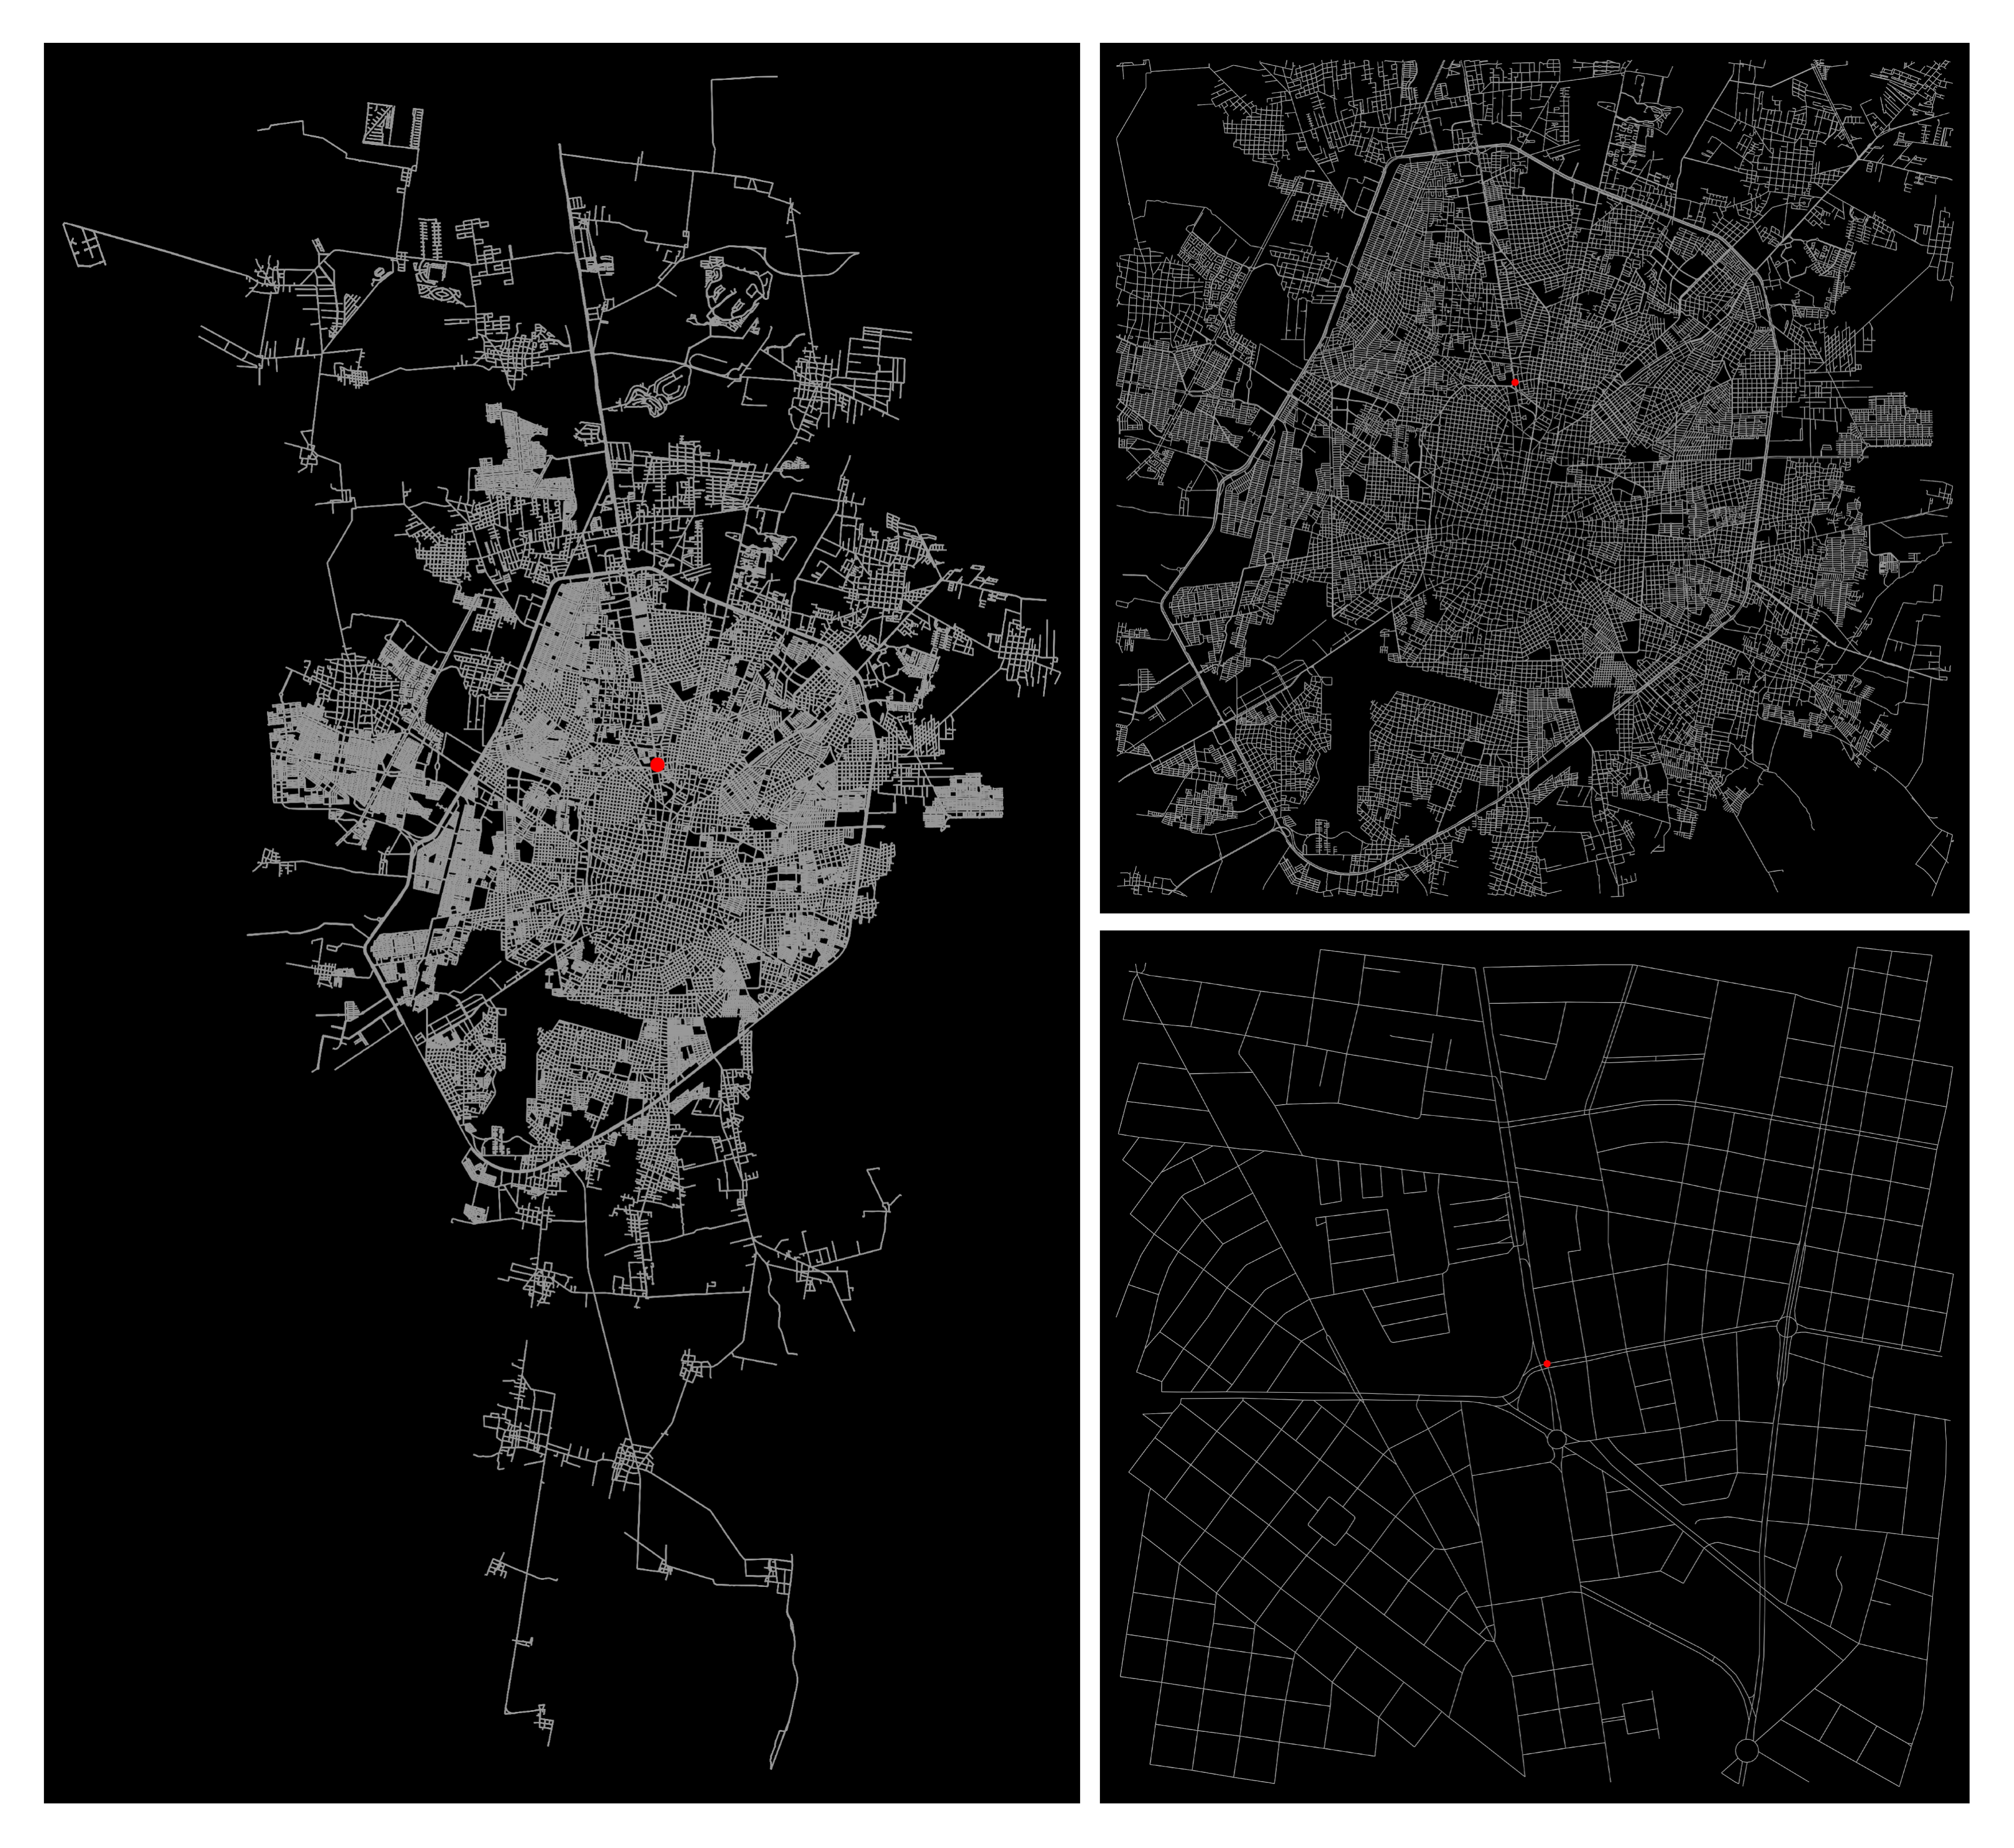
\includegraphics[width=0.8\textwidth]{Figures/merida-node-closeness-centrality.png}
	\caption{Node with highest closeness centrality score. This node is located at the Circuito Colonias and 60 street.
		\label{fig:merida-max-node-closeness-centrality}}
\end{figure}

\begin{figure}[h!]
	\centering
	\includegraphics[width=0.5\textwidth]{Figures/merida-closeness-centrality.png}
	\caption{Closeness centrality of all nodes in Mérida. Nodes are visualized from low (dark violet) to high (light yellow).
		\label{fig:merida-closeness-centrality}}
\end{figure}

\begin{figure}[h!]
	\centering
	\includegraphics[width=0.5\textwidth]{Figures/merida-edge-closeness-centrality.png}
	\caption{Closeness centrality of all edges in Mérida. Edges are visualized from low (dark) to high (light yellow).
		\label{fig:merida-edge-closeness-centrality}}
\end{figure}

Betweenness centrality declares that important nodes are those who connect other nodes; it is also a measure to examine resilience in the network. In Mérida, the node highlighted in red has approximately 7\% of all shortest paths running through it (see Figure \ref{fig:merida-max-node-betweenness-centrality}). If we observe Figure \ref{fig:merida-betweenness-centrality}, see that intersection in principal avenues and streets are the most important, which makes sense because they connect the city in a more efficient way.

\begin{figure}[h!]
	\centering
	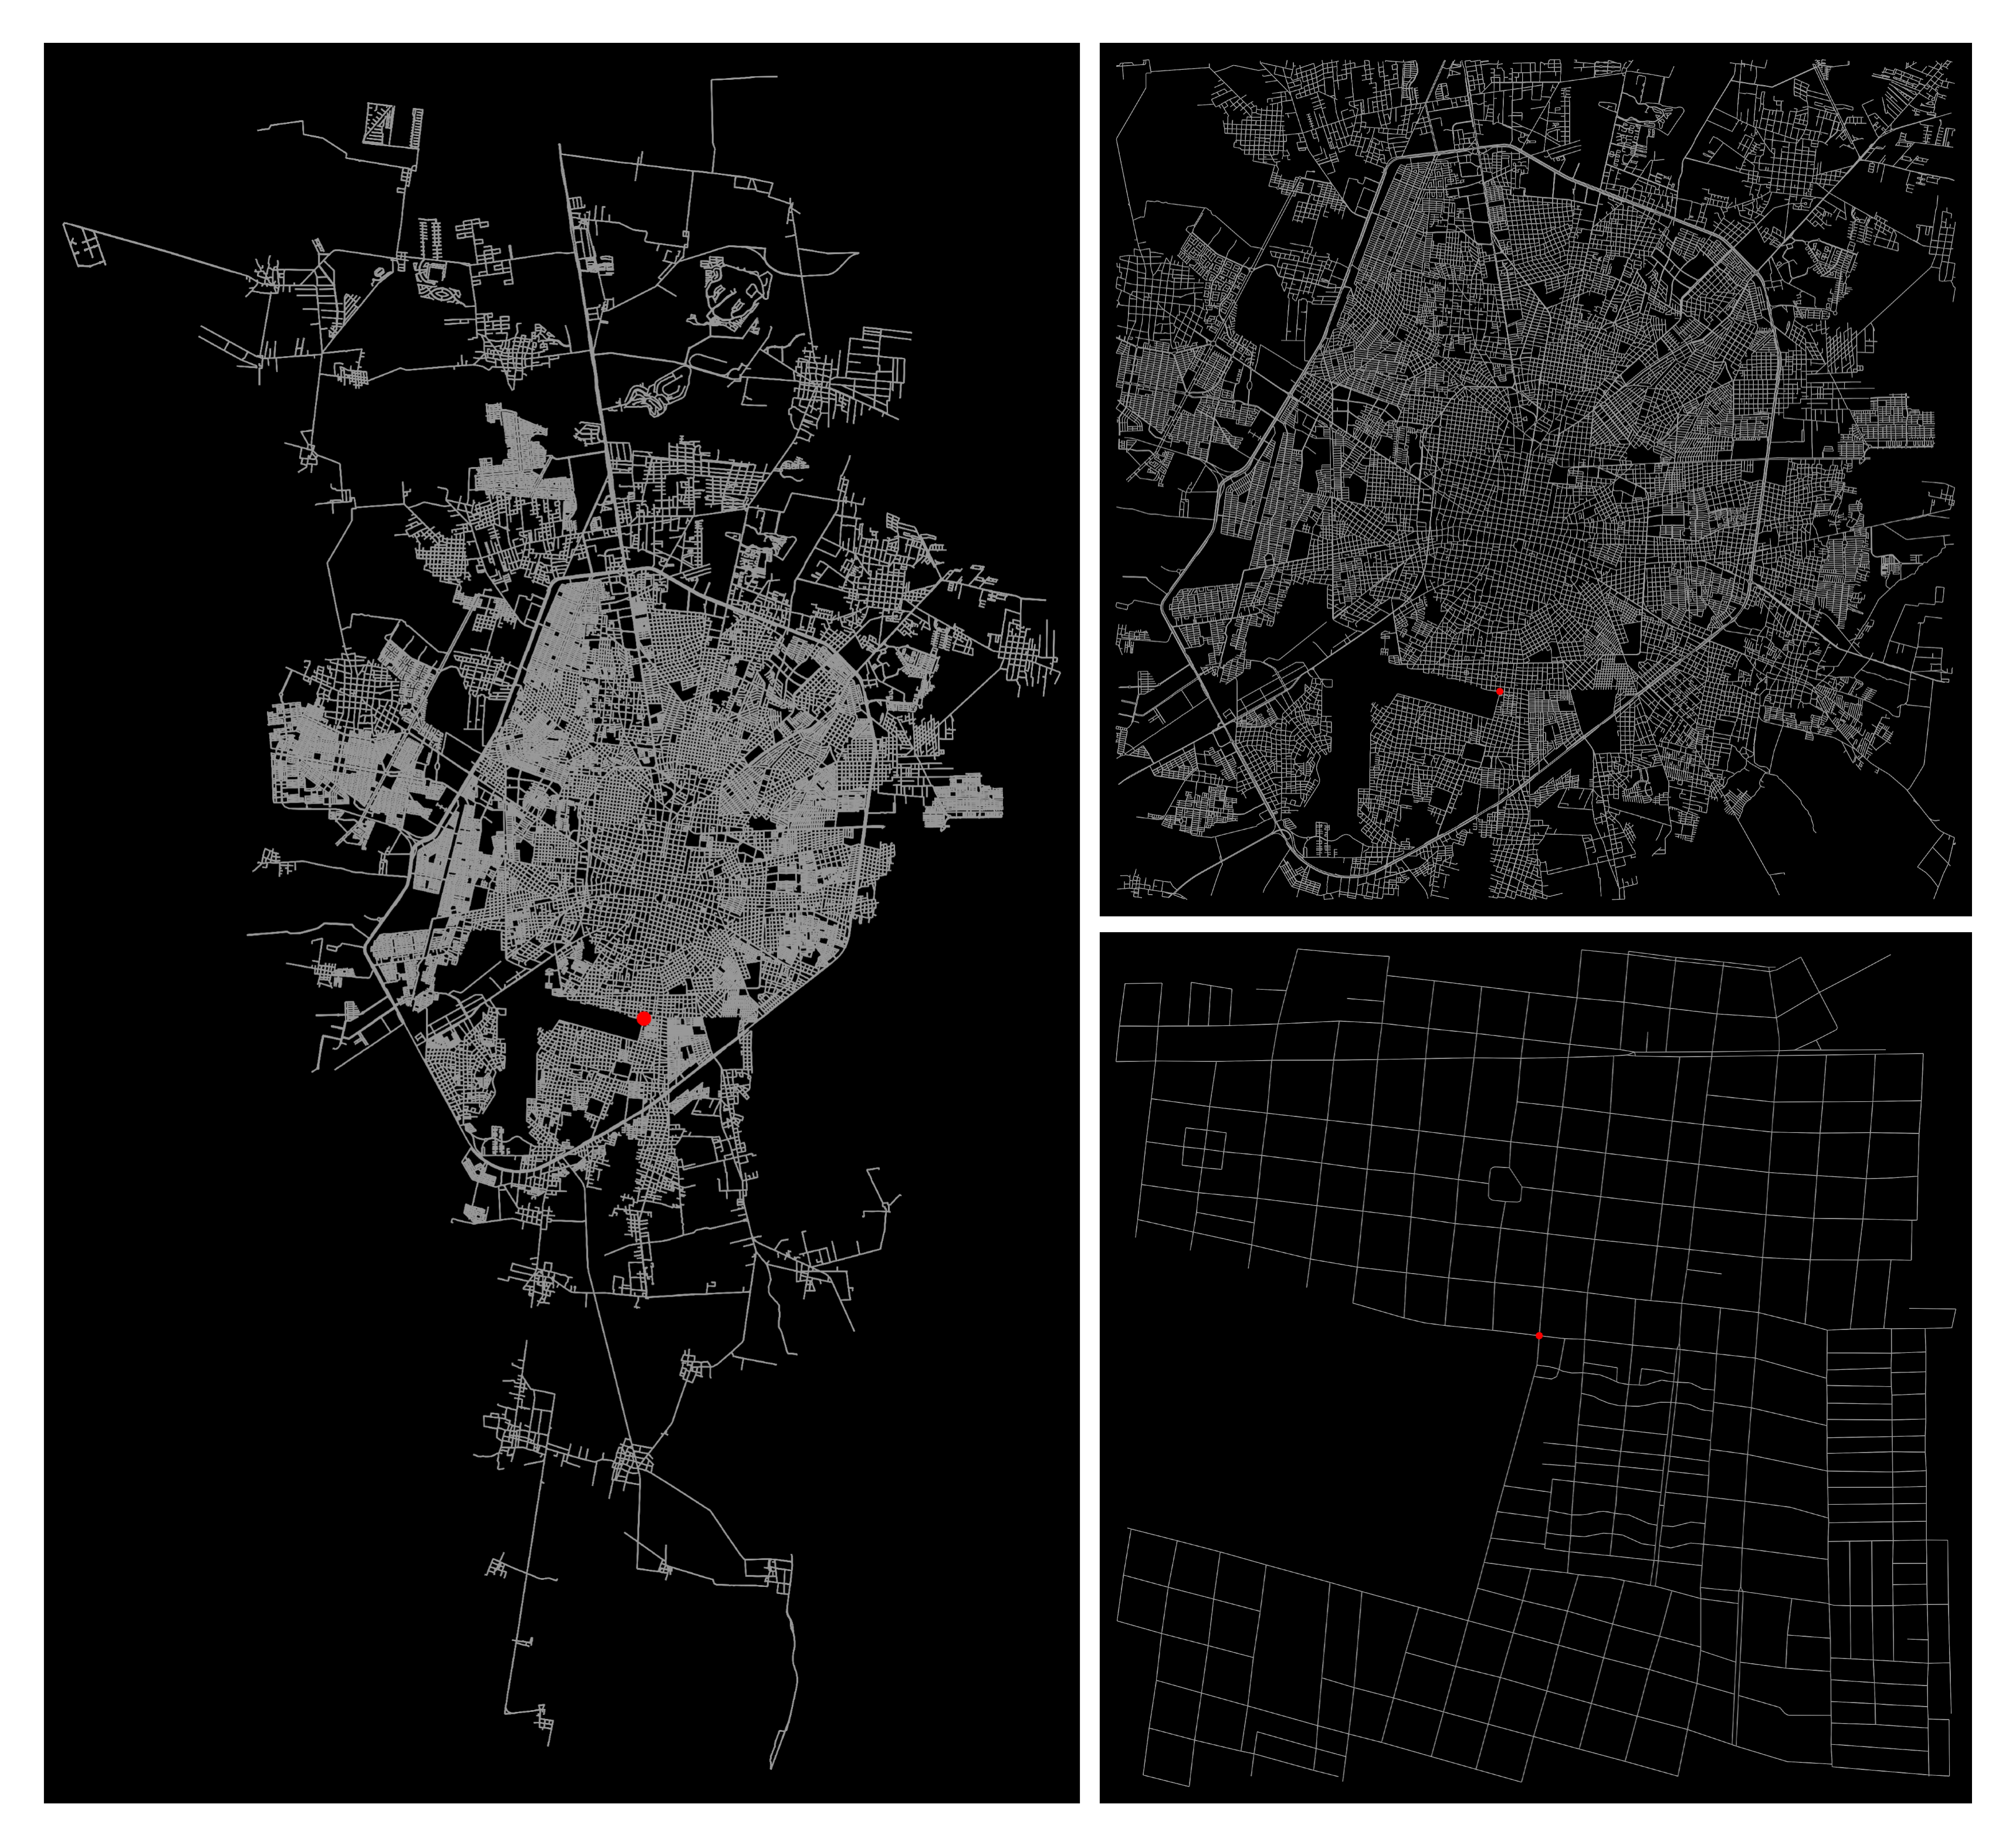
\includegraphics[width=0.8\textwidth]{Figures/merida-node-betweenness-centrality.png}
	\caption{Node with highest betweenness centrality score. This node is the intersection at 121 street and 54 street, colonia Mercedes Barrera.
		\label{fig:merida-max-node-betweenness-centrality}}
\end{figure}

\begin{figure}[h!]
	\centering
	\includegraphics[width=0.5\textwidth]{Figures/merida-betweenness-centrality.png}
	\caption{Betweenness centrality of all nodes in Mérida. Nodes are visualized from low (dark violet) to high (light yellow).
		\label{fig:merida-betweenness-centrality}}
\end{figure}

Finally, PageRank makes the assumption that important nodes are those that have many in-links from other important nodes; this measure is useful for directed networks. The node with highest PageRank is presented in Figure \ref{fig:merida-max-node-pagerank}. This node is important because it is connected to other important nodes, which makes sense because it is located at one of the most important avenues in Mérida city.

\begin{figure}[h!]
	\centering
	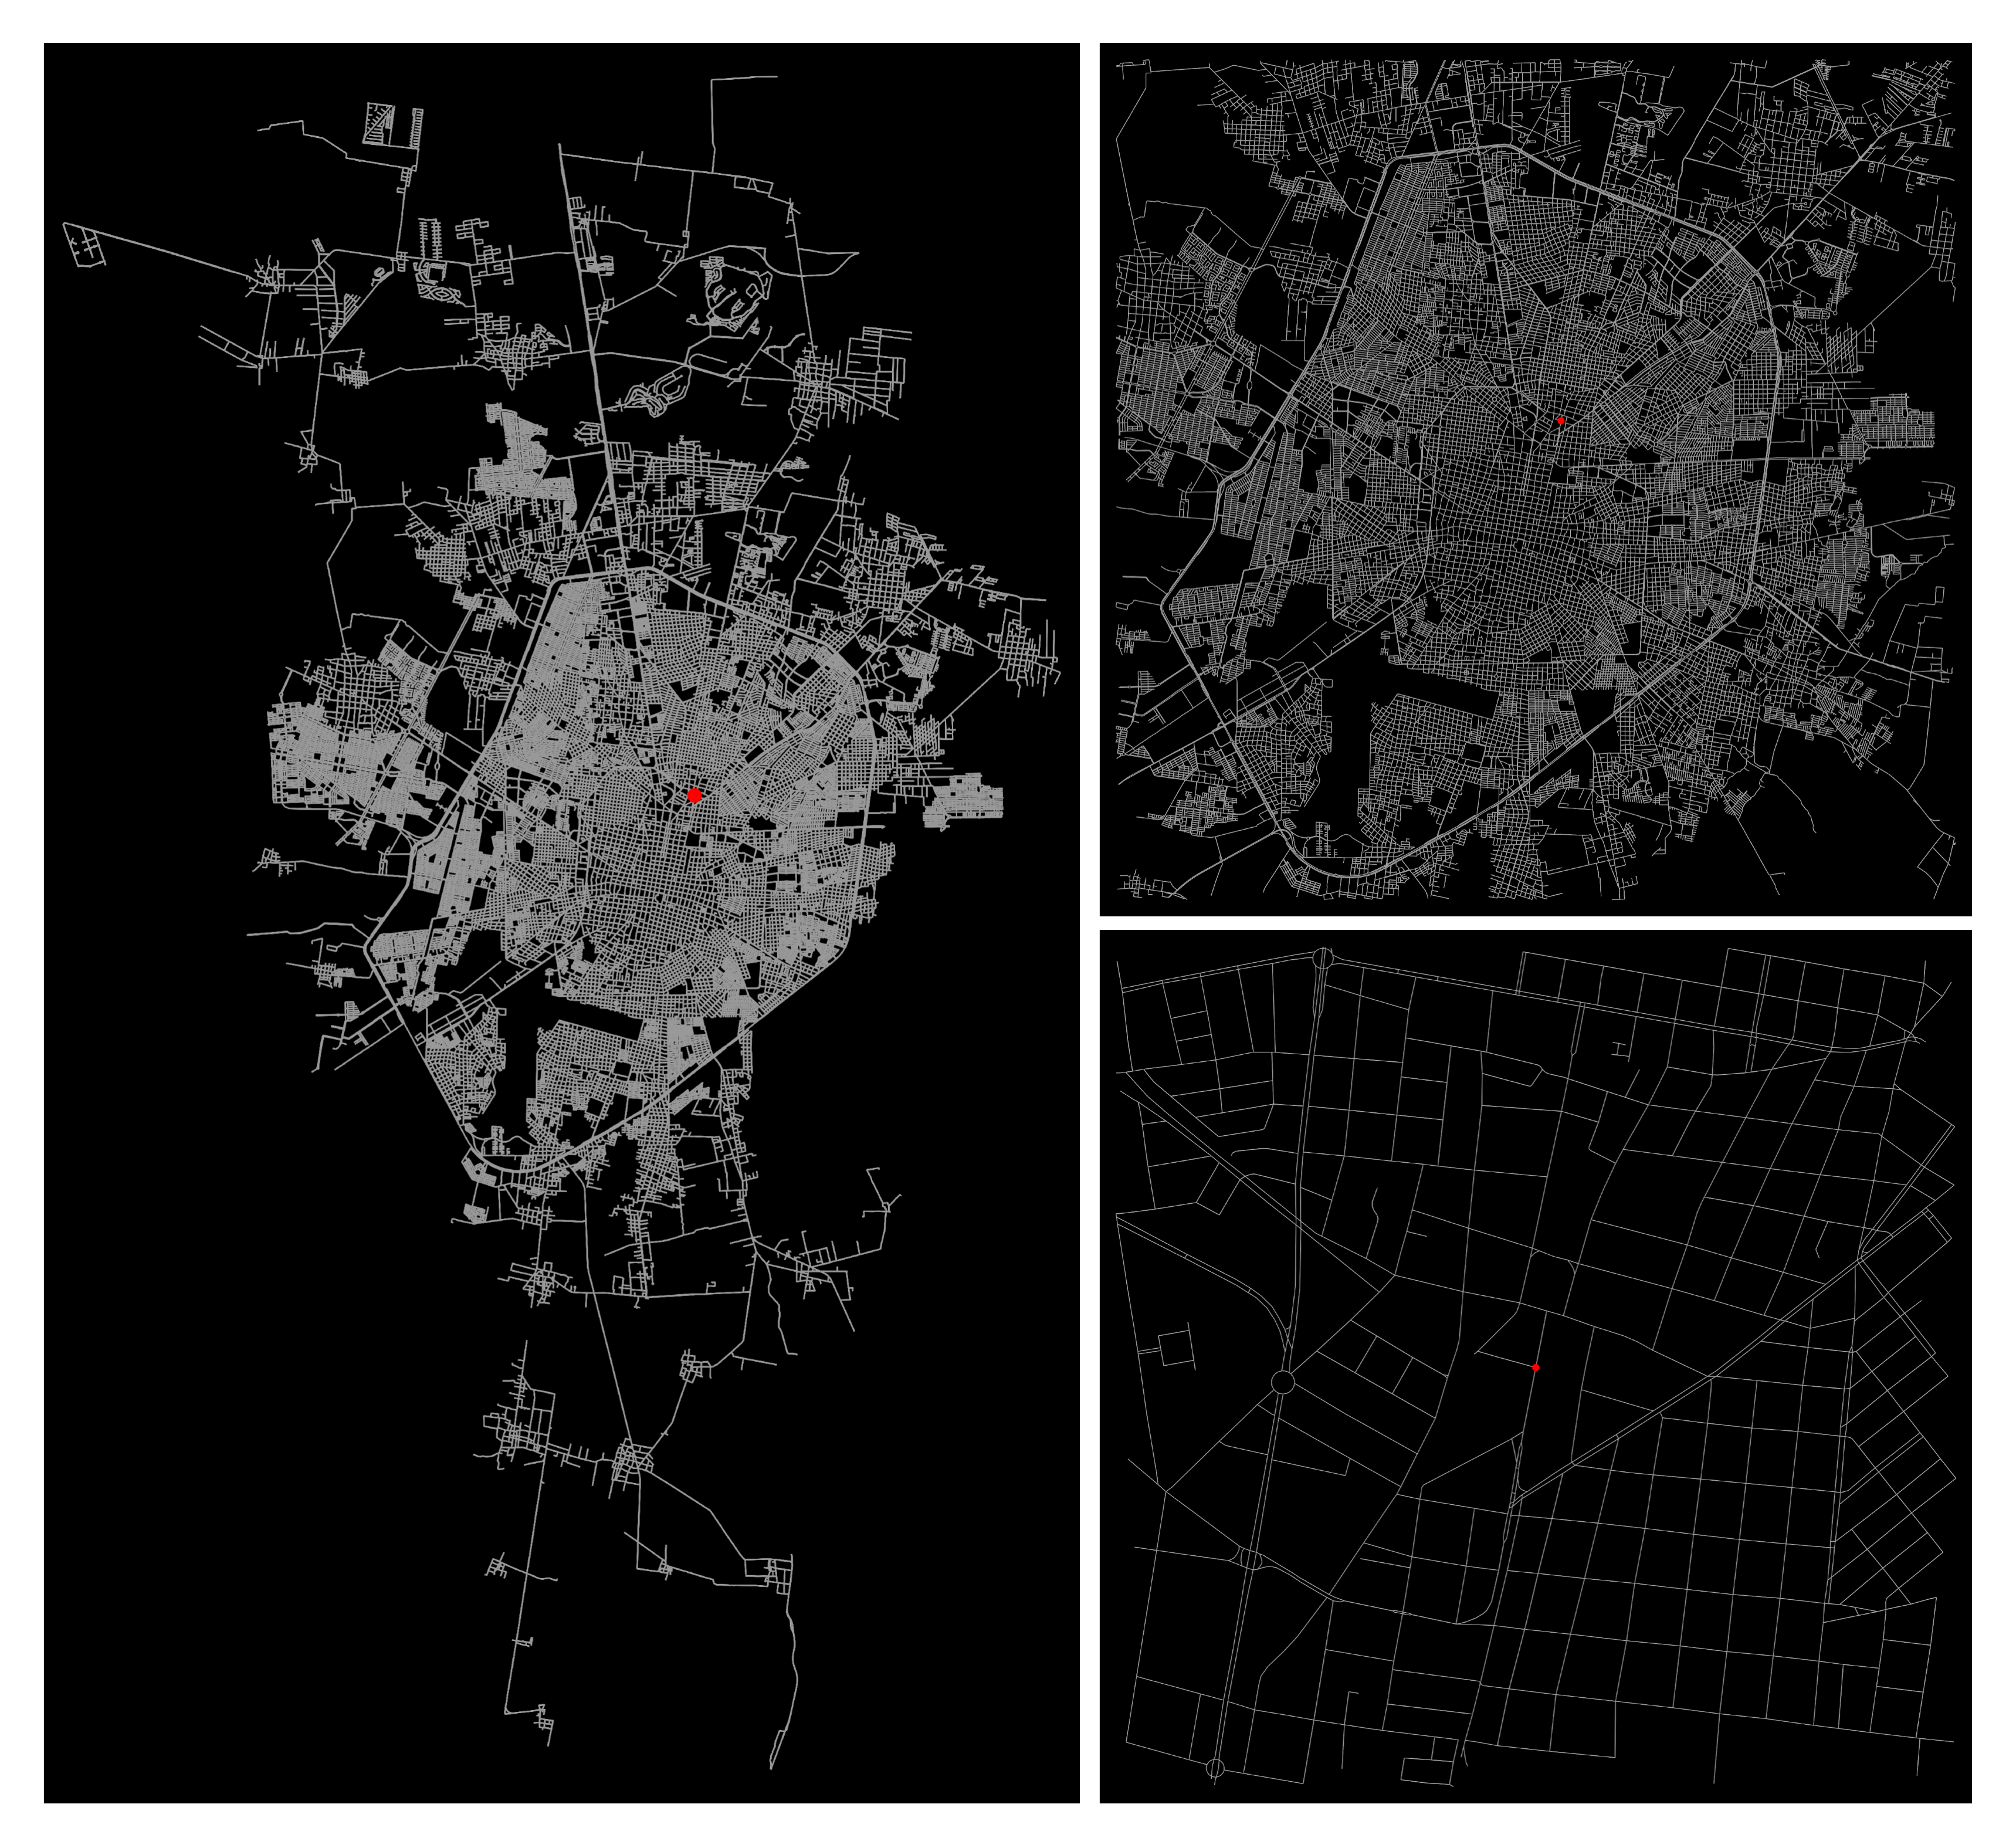
\includegraphics[width=0.8\textwidth]{Figures/merida-node-pagerank.png}
	\caption{Node with highest PageRank score. This node is located at Rotary Internacional Av. and 21A street, colonia Itzimna.
		\label{fig:merida-max-node-pagerank}}
\end{figure}

\section{AGEB scale}

While the municipal scale captures planning decisions made by the city government, the neighborhood, or, in this case, AGEB represent the scale of individual urban design intervertions into the urban form \cite{boeing_multi-scale_2018}. Additionally, this scale reflects the street network development in different eras, designs, and paradigms individually.

Table \ref{tab:measures_urban_agebs} presents summary statistics for the 513 AGEBs used in this work. The typical AGEB has 3.2 streets per intersection (see Figure \ref{fig:merida-ageb-histograms}a), reflecting the prevalence of 3-way intersections in the municipality, discussed earlier. The median proportions of each node type are 3.1\% for dead-ends, 58.5\% for 3-way intersections, and 34.9\% for 4-way intersections. The typical AGEB averages 92-meter street segment lengths (Figure \ref{fig:merida-ageb-histograms}b) and 112.8 intersections per km$^2$ (Figure \ref{fig:merida-ageb-histograms}c).


\begin{table*}[htbp]
	\centering
	\caption{Central tendency and statistical dispersion for selected measures of all Mérida urban AGEB's street networks: $\mu$ is the mean, $\sigma$ is the standard deviation, and $D$ is the dispersion index $\frac{\sigma ^ 2}{\mu}$.}
	\label{tab:measures_urban_agebs}
	\small
	\begin{tabular}{ l r r r r r r }
		\toprule
		measure                                          & $\mu$          & $\sigma$       & min            & median         & max            & $D$            \\
		\midrule
		Area (km\textsuperscript{2})                     & 0.582        & 0.527        & 0.014         & 0.475        & 7.613       & 0.477       \\
		Avg of the avg neighborhood degree               & 2.477          & 0.470          & 0.500          & 2.556          & 3.414          & 0.089          \\
		Avg of the avg weighted neighborhood degree      & 0.039          & 0.012          & 0.005          & 0.039          & 0.097          & 0.004          \\
		Avg circuity                                     & 0.960          & 0.066          & 0.932          & 0.940          & 1.741          & 0.005 \\
		Avg clustering coefficient                       & 0.027          & 0.044          & 0          & 0.017          & 0.583          & 0.072          \\
		Avg weighted clustering coefficient              & 0.007          & 0.02          & 0 & 0.003          & 0.397          & 0.057 \\
		Intersection count                               & 53.393          & 29.065          & 1            & 52           & 204         & 15.664      \\
		Avg degree centrality                            & 0.156          & 0.270          & 0.015 & 0.088          & 2          & 0.467          \\
		Edge density (km/km\textsuperscript{2})          & 23657.180         & 8967.089          & 1543.392          & 23866.890         & 47341.220         & 3398.913          \\
		Avg edge length (m)                              & 92.625        & 23.339         & 44.488        & 88.761        & 237.350        & 5.881          \\
		Total edge length (km)                           & 12.153           & 7.015          & 0.01            & 11.47           & 49.218         & 4.05      \\
		Proportion of dead-ends                          & 0.069          & 0.089          & 0          & 0.031          & 0.500          & 0.115          \\
		Proportion of 3-way intersections                & 0.566          & 0.179          & 0          & 0.585          & 1          & 0.057          \\
		Proportion of 4-way intersections                & 0.373          & 0.190          & 0.006          & 0.349          & 1          & 0.097          \\
		Intersection density (per km\textsuperscript{2}) & 112.849         & 54.826          & 8.403         & 108.692         & 410.011         & 26.636          \\
		Average node degree                              & 1.348          & 0.488          & 0.163          & 1.333          & 2.772          & 0.177          \\
		$m$                                              & 136.035          & 11.534          & 2           & 130          & 528         & 44.191     \\
		$n$                                              & 58.193          & 33.431          & 2            & 54           & 264         & 19.206      \\
		Node density (per km\textsuperscript{2})         & 120.451         & 57.043          & 9.226         & 116.253         & 410.011         & 27.014          \\
		Max PageRank value                               & 0.063          & 0.082          & 0.001 & 0.039          & 0.500          & 0.107 \\
		Min PageRank value                               & 0.016 & 0.060 & 0.001 & 0.003 & 0.500 & 0.225 \\
		Self-loop proportion                             & 0.001          & 0.004          & 0 & 0          & 0.046          & 0.016         \\
		Street density (km/km\textsuperscript{2})        & 13743.660          & 4999.535          & 774.708          & 13920.640          & 28345.930         & 1818.683          \\
		Average street segment length (m)                & 92.472        & 22.521         & 44.488        & 88.585        & 198.010        & 5.485          \\
		Total street length (km)                         & 7.134           & 4.120           & 0.045            & 6.750           & 32.542          & 2.375      \\
		Street segment count                             & 79.803          & 45.775          & 1           & 76           & 321         & 26.257      \\
		Average streets per node                         & 3.225          & 0.320          & 2          & 3.25          & 4          & 0.032          \\
		\bottomrule
	\end{tabular}
\end{table*}

\begin{figure}[h!]
	\centering
	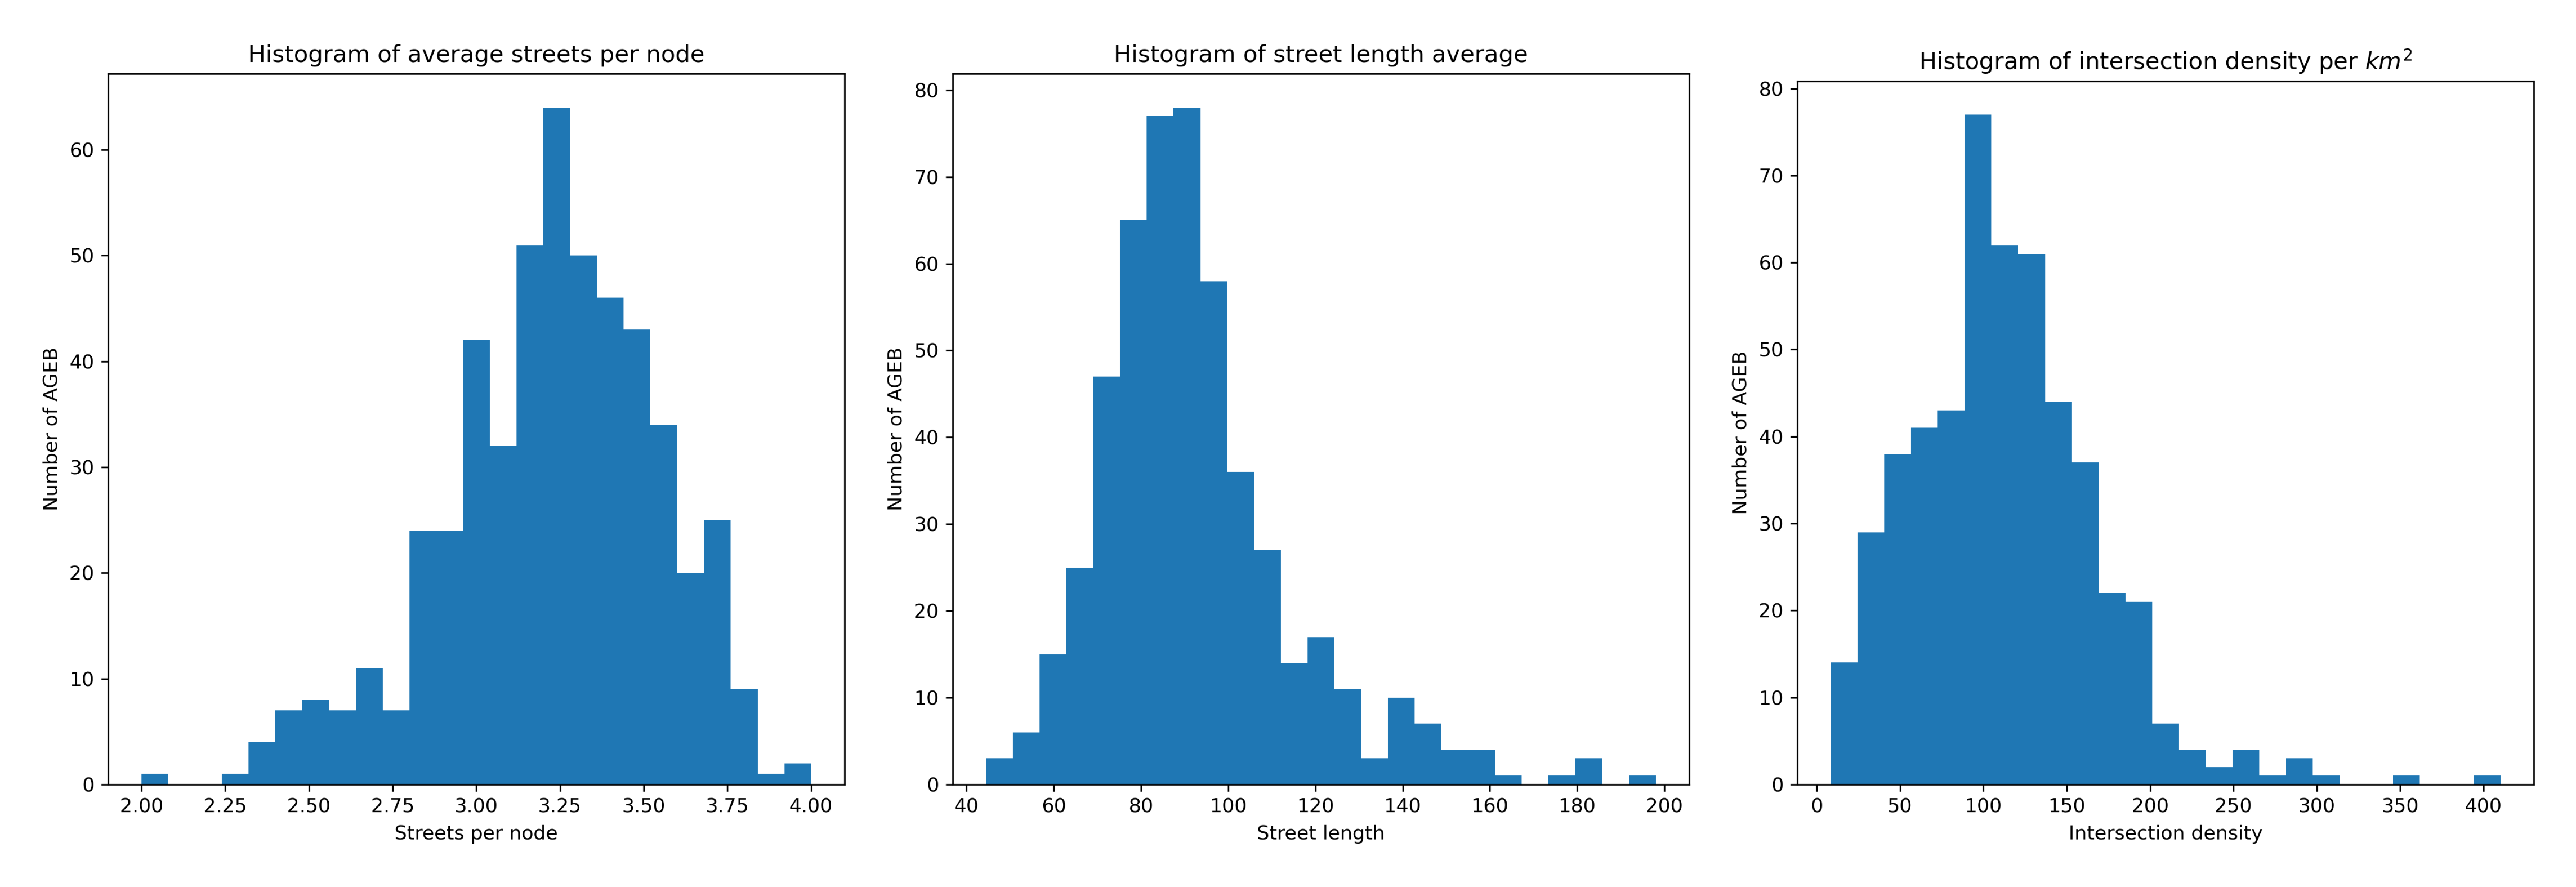
\includegraphics[width=\textwidth]{Figures/merida-ageb-histograms.png}
	\caption{Histograms of average streets per node (left), average street length (middle), and intersection density per km$^2$ (right).
		\label{fig:merida-ageb-histograms}}
\end{figure}

In Figure \ref{fig:merida-ageb-street-length-vs-nodes} , we examine the relationship between the total street length and the number of nodes across the AGEBs, and we find a meaningful linear relationship ($r^2 = 0.81$). The not-so-strong linear relationship is due to the fact that we are handling invariant street networks designed and shaped in different historical eras.

\begin{figure}[h!]
	\centering
	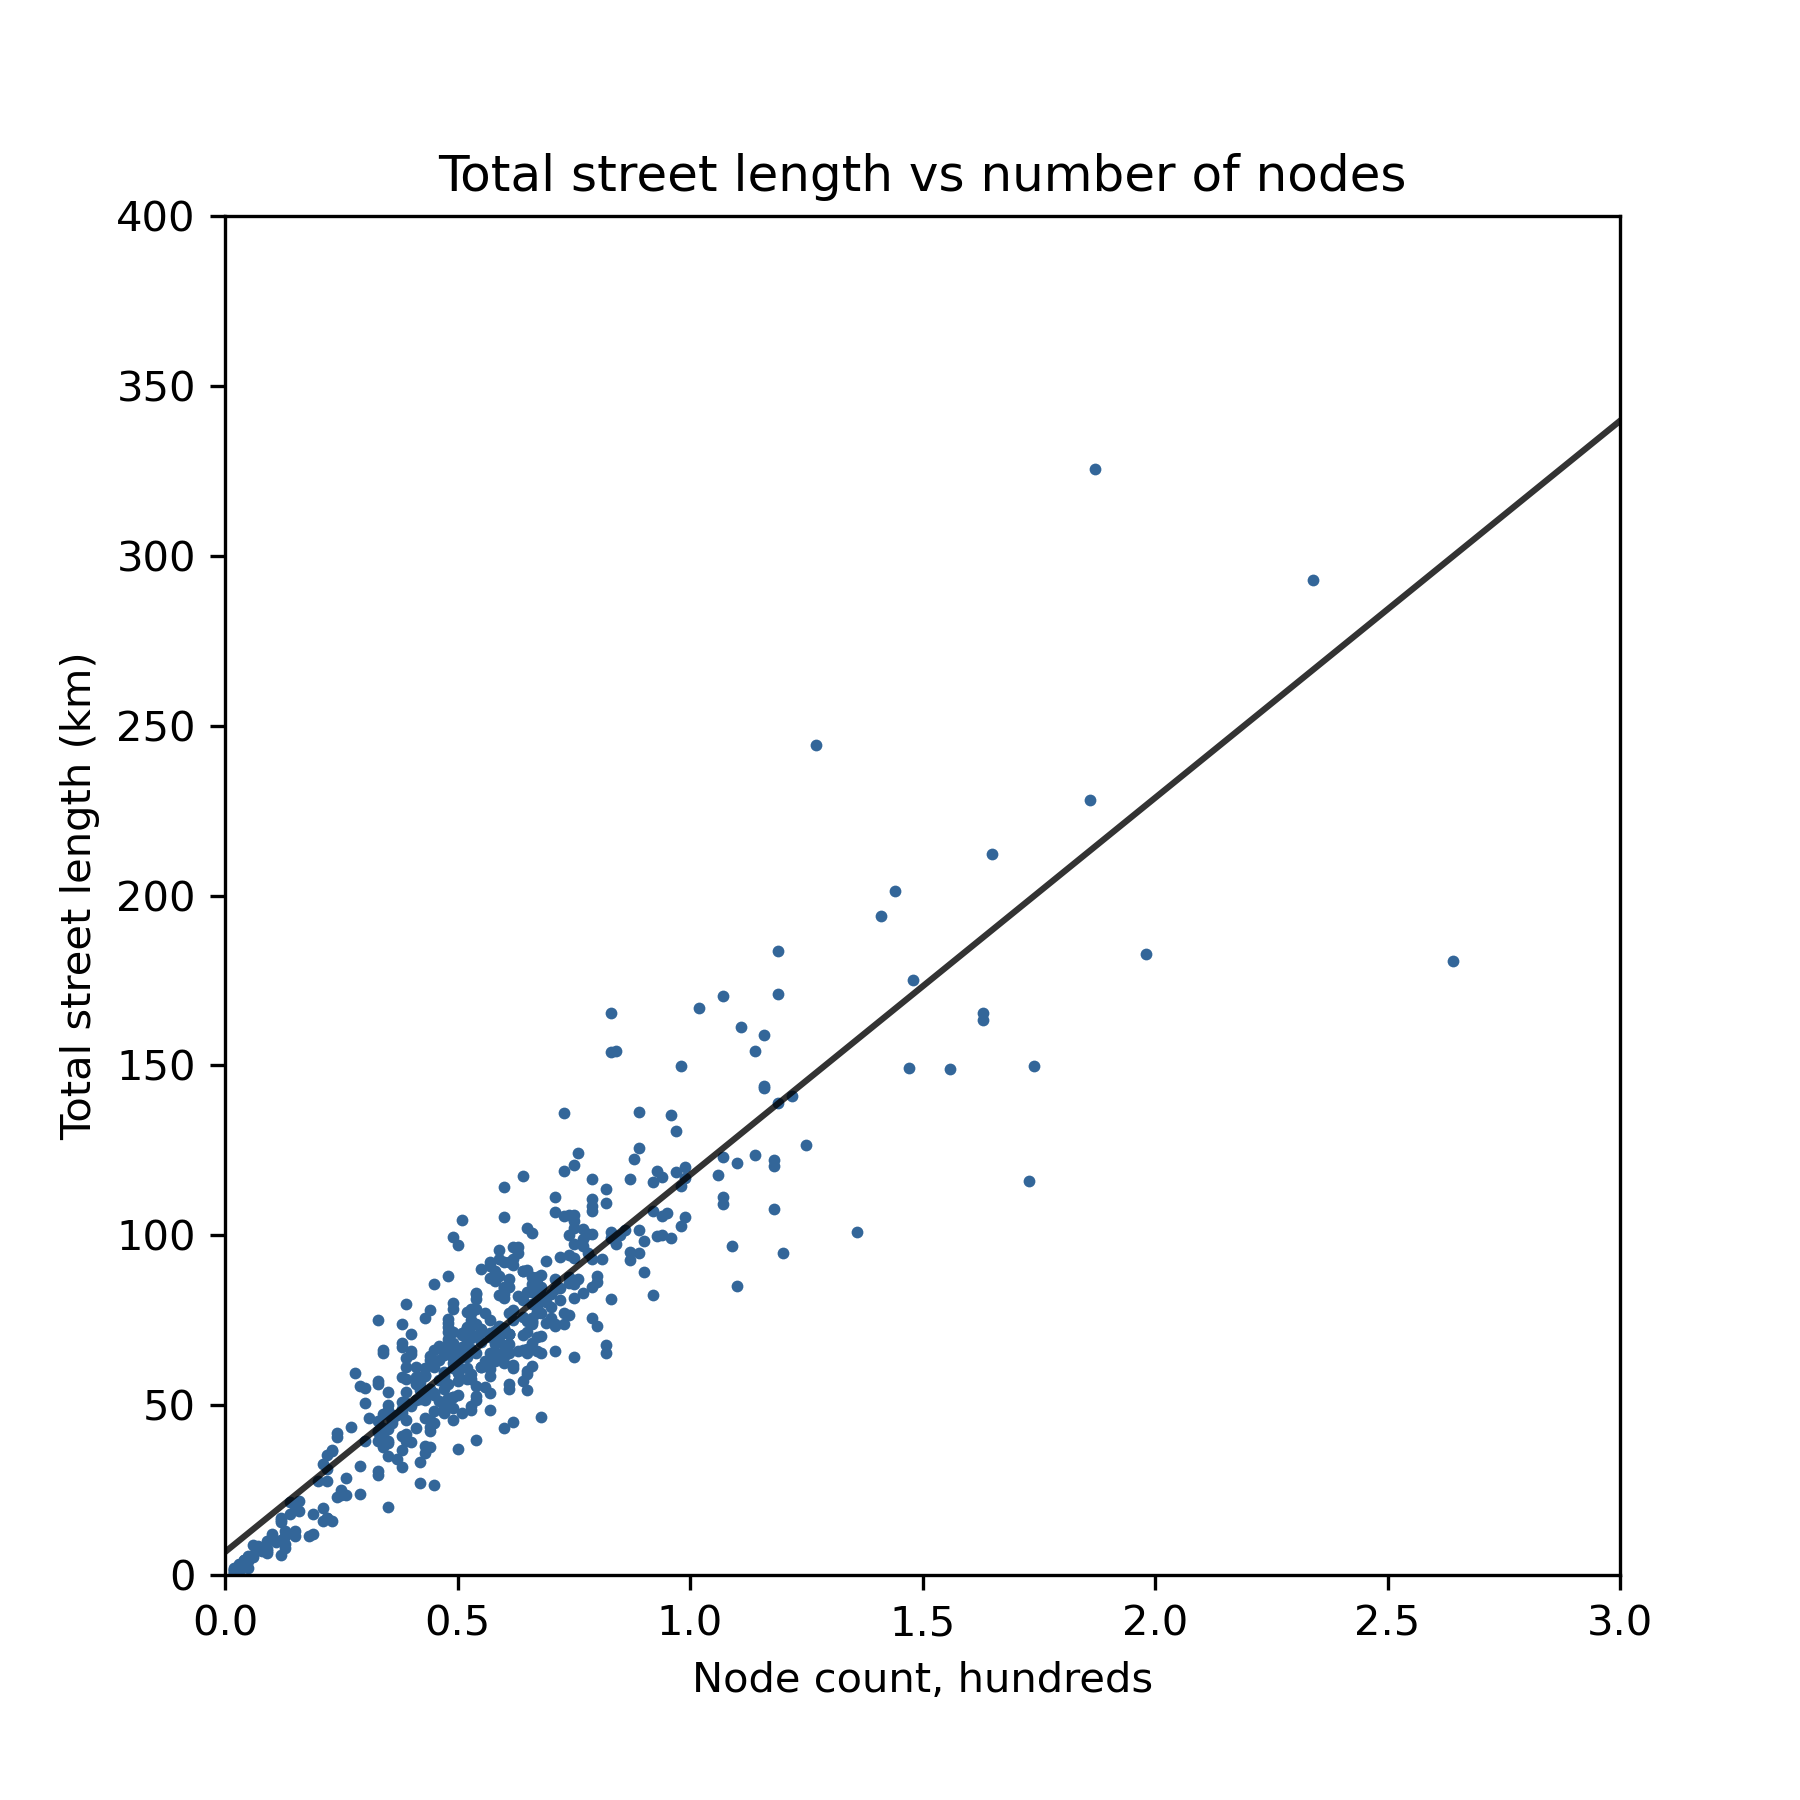
\includegraphics[width=0.5\textwidth]{Figures/merida-ageb-street-length-vs-nodes.png}
	\caption{Linear relationship between total street length and number of nodes in the street network of every Mérida urban AGEB.
		\label{fig:merida-ageb-street-length-vs-nodes}}
\end{figure}

Figure \ref{fig:merida-ageb-avg-street-length} depicts the mean street length by AGEB. We can observe that the greatest average street lengths tend to be in older AGEBs such as those in the historical center of Mérida, also outside the boundary of the city, and, more specifically, in towns such as Caucel Pueblo, Komchen, Chablekal, Cholul, and San José Tzal. On the other hand, he lowest average street lengths are present in new residential lands. This attribute is a useful factor for studying the dynamics of the municipality during its different development eras.

\begin{figure}[h!]
	\centering
	\includegraphics[width=0.5\textwidth]{Figures/merida-ageb-avg-street-length.png}
	\caption{Map AGEB by average street length. AGEBs are visualized from low (dark) to high (light yellow). The colors in colorspace are linearly mapped to the attribute values.
		\label{fig:merida-ageb-avg-street-length}}
\end{figure}

Looking at Figure \ref{fig:merida-ageb-betweenness}, we can observe that the most important (light-yellow colored) AGEBs are in non-concurrent locations (one or two in every town of the municipality) because betweenness centrality is measuring resilience in the network and identifies important AGEBs as the more prone to failure or inefficiency since a large number of shortest paths rely on them. 

\begin{figure}[h!]
	\centering
	\includegraphics[width=0.5\textwidth]{Figures/merida-ageb-betweenness.png}
	\caption{Map AGEB by mean betweenness centrality. AGEBs are visualized from low (dark) to high (light yellow).
		\label{fig:merida-ageb-betweenness}}
\end{figure}

\section{Clustering}

Assigned clusters give us a clearer view of how the municipality is subdivided (see Figure \ref{fig:merida-ageb-clusters}). In clusters 0 and 11, we can observe the division from Caucel City (cluster 0) to Caucel Pueblo (cluster 11), which is mostly defined by their topological characteristics such as the average street length, being cluster 11 with the highest. Cluster 9 includes the historical center, being the oldest roads of Mérida. Clusters 2 and 12 can be differentiated by the street design. Cluster 12 has higher intersection density per km$^2$. AGEBs in cluster 10 belong to the Cuxtal Ecological Reserve.

We can start noticing the differences based on socio-demographic data by contrasting clusters 2 with 6, and clusters 1 with 6. The clustering algorithm defines very well two different residential lands: cluster 5 being Las Américas, and cluster 8 being Los Héroes. Both of them have different economic differences: people in the former tend to be of a higher economic status than the latter.

Cluster 3 belongs to the town of Cholul, which also contains AGEBs with small residential lands. In cluster 7 there are factories and industrial companies rather than people living in there; also, it has low intersection density. Low intersection density is also present in clusters 4 and 13. However, both clusters are different in the amount of people and number of streets. The former has twice the people and three times the streets than the latter.

\begin{figure}[h!]
	\centering
	\includegraphics[width=0.5\textwidth]{Figures/merida-ageb-clusters-rook.png}
	\caption{Map AGEB by clusters. Each colored cluster is labeled from 0 to 13 in the centroid of the unary union of AGEBs' area from the same cluster.
		\label{fig:merida-ageb-clusters}}
\end{figure}


\chapter{Conclusions and recommendations}
\label{cha:conclusions}
\section{Conclusion}


\section{Recommendations}


%now enable appendix numbering format and include any appendices
%\appendix
%\include{content/appendix1}

\addcontentsline{toc}{chapter}{Bibliography}
\bibliography{refs}        %use a bibtex bibliography file refs.bib
\bibliographystyle{unsrt}

\end{document}


%%% Local Variables:
%%% mode: latex
%%% TeX-master: t
%%% End:
